% !Mode:: "TeX:UTF-8"
%# -*- coding:utf-8 -*-

%% 使用 njuthesis 文档类生成南京大学学位论文的示例文档
%%作者:njuhan: https://github.com/njuHan
%% 部分提纲取自njuhan的本科毕业论文

\documentclass[winfonts,master,oneside,nobackinfo]{njuthesis}
%% njuthesis 文档类的可选参数有:
%%   nobackinfo 取消封二页导师签名信息。注意,按照南大的规定,是需要签名页的。
%%   phd/master/bachelor 选择博士/硕士/学士论文

\usepackage{float}
\usepackage{lipsum}
\usepackage{listings}
\usepackage{xcolor}
\usepackage{algorithm}
\usepackage{algorithmic}
\lstset{breaklines}%这条命令可以让LaTeX自动将长的代码行换行排版
\lstset{extendedchars=false}%这一条命令可以解决代码跨页时,章节标题,页眉等汉字不显示的问题
\lstset{                        %Settings for listings package.
  language=[ANSI]{C},
  backgroundcolor=\color{white},
  basicstyle=\footnotesize,
  breakatwhitespace=false,
  breaklines=true,
  captionpos=b,
  commentstyle=\color{olive},
  directivestyle=\color{blue},
  extendedchars=false,
  % frame=single,%shadowbox
  framerule=0pt,
  keywordstyle=\color{blue}\bfseries,
  morekeywords={*,define,*,include...},
  numbersep=5pt,
  rulesepcolor=\color{red!20!green!20!blue!20},
  showspaces=false,
  showstringspaces=false,
  showtabs=false,
  stepnumber=2,
  stringstyle=\color{purple},
  tabsize=4,
  title=\lstname
}


%%%%%%%%%%%%%%%%%%%%%%%%%%%%%%%%%%%%%%%%%%%%%%%%%%%%%%%%%%%%%%%%%%%%%%%%%%%%%%%
% 设置《国家图书馆封面》的内容,仅博士论文才需要填写

% 设置论文按照《中国图书资料分类法》的分类编号
\classification{0175.2}
% 论文的密级。需按照GB/T 7156-2003标准进行设置。预定义的值包括:
% - \openlevel,表示公开级:此级别的文献可在国内外发行和交换。
% - \controllevel,表示限制级:此级别的文献内容不涉及国家秘密,但在一定时间内
%   限制其交流和使用范围。
% - \confidentiallevel,表示秘密级:此级别的文献内容涉及一般国家秘密。
% - \clasifiedlevel,表示机密级:此级别的文献内容涉及重要的国家秘密 。
% - \mostconfidentiallevel,表示绝密级:此级别的文献内容涉及最重要的国家秘密。
% 此属性可选,默认为\openlevel,即公开级。
\securitylevel{\controllevel}
% 设置论文按照《国际十进分类法UDC》的分类编号
% 该编号可在下述网址查询:http://www.udcc.org/udcsummary/php/index.php?lang=chi
\udc{004.72}
% 国家图书馆封面上的论文标题第一行,不可换行。此属性可选,默认值为通过\title设置的标题。
\nlctitlea{数据中心}
% 国家图书馆封面上的论文标题第二行,不可换行。此属性可选,默认值为空白。
\nlctitleb{网络模型研究}
% 国家图书馆封面上的论文标题第三行,不可换行。此属性可选,默认值为空白。
\nlctitlec{}
% 导师的单位名称及地址
\supervisorinfo{南京大学计算机科学与技术系~~南京市汉口路22号~~210093}
% 答辩委员会主席
\chairman{张三丰~~教授}
% 第一位评阅人
\reviewera{阳顶天~~教授}
% 第二位评阅人
\reviewerb{张无忌~~副教授}
% 第三位评阅人
\reviewerc{黄裳~~教授}
% 第四位评阅人
\reviewerd{郭靖~~研究员}


%%%%%%%%%%%%%%%%%%%%%%%%%%%%%%%%%%%%%%%%%%%%%%%%%%%%%%%%%%%%%%%%%%%%%%%%%%%%%%%
% 设置论文的中文封面

% 论文标题,不可换行
\title{南大本科毕业论文\LaTeX 模板}
% 如果论文标题过长,可以分两行,第一行用\titlea{}定义,第二行用\titleb{}定义,将上面的\title{}注释掉
% \titlea{半轻衰变$D^+\to \omega(\phi)e^+\nu_e$的研究}
% \titleb{和弱衰变$J/\psi \to D_s^{(*)-}e^+\nu_e$的寻找}

% 论文作者姓名
\author{作者}
% 论文作者联系电话
\telphone{xxxx}
% 论文作者电子邮件地址
\email{sample@smail.nju.edu.cn}
% 论文作者学生证号
\studentnum{12xxxxxxx}
% 论文作者入学年份(年级)
\grade{2012}
% 导师姓名职称
\supervisor{某~~教授}
% 导师的联系电话
\supervisortelphone{}
% 论文作者的学科与专业方向
\major{计算机科学与技术}
% 论文作者的研究方向
\researchfield{分布式计算}
% 论文作者所在院系的中文名称
\department{计算机科学与技术系}
% 论文作者所在学校或机构的名称。此属性可选,默认值为``南京大学''。
\institute{南京大学}
% 论文的提交日期,需设置年、月、日。
\submitdate{2016年\qquad 月\qquad 日}
% 论文的答辩日期,需设置年、月、日。
\defenddate{2016年\qquad 月\qquad 日}
% 论文的定稿日期,需设置年、月、日。此属性可选,默认值为最后一次编译时的日期,精确到日。
\date{2016年6月8日}

%%%%%%%%%%%%%%%%%%%%%%%%%%%%%%%%%%%%%%%%%%%%%%%%%%%%%%%%%%%%%%%%%%%%%%%%%%%%%%%
% 设置论文的英文封面

% 论文的英文标题,不可换行
\englishtitle{\LaTeX \;  NJU thesis template }
% 论文作者姓名的拼音
\englishauthor{Author}
% 导师姓名职称的英文
\englishsupervisor{ Professor}
% 论文作者学科与专业的英文名
\englishmajor{Computer Science and Technology}
% 论文作者所在院系的英文名称
\englishdepartment{Department of Computer Science and Technology}
% 论文作者所在学校或机构的英文名称。此属性可选,默认值为``Nanjing University''。
\englishinstitute{Nanjing University}
% 论文完成日期的英文形式,它将出现在英文封面下方。需设置年、月、日。日期格式使用美国的日期
% 格式,即``Month day, year'',其中``Month''为月份的英文名全称,首字母大写;``day''为
% 该月中日期的阿拉伯数字表示;``year''为年份的四位阿拉伯数字表示。此属性可选,默认值为最后
% 一次编译时的日期。
\englishdate{May 20th, 2016}

%%%%%%%%%%%%%%%%%%%%%%%%%%%%%%%%%%%%%%%%%%%%%%%%%%%%%%%%%%%%%%%%%%%%%%%%%%%%%%%
% 设置论文的中文摘要

% 设置中文摘要页面的论文标题及副标题的第一行。
% 此属性可选,其默认值为使用|\title|命令所设置的论文标题
% \abstracttitlea{数据中心网络模型研究}
% 设置中文摘要页面的论文标题及副标题的第二行。
% 此属性可选,其默认值为空白
% \abstracttitleb{}

%%%%%%%%%%%%%%%%%%%%%%%%%%%%%%%%%%%%%%%%%%%%%%%%%%%%%%%%%%%%%%%%%%%%%%%%%%%%%%%
% 设置论文的英文摘要

% 设置英文摘要页面的论文标题及副标题的第一行。
% 此属性可选,其默认值为使用|\englishtitle|命令所设置的论文标题
\englishabstracttitlea{englishabstracttitlea}
% 设置英文摘要页面的论文标题及副标题的第二行。
% 此属性可选,其默认值为空白
\englishabstracttitleb{nglishabstracttitleb}

%%%%%%%%%%%%%%%%%%%%%%%%%%%%%%%%%%%%%%%%%%%%%%%%%%%%%%%%%%%%%%%%%%%%%%%%%%%%%%%
\begin{document}

%%%%%%%%%%%%%%%%%%%%%%%%%%%%%%%%%%%%%%%%%%%%%%%%%%%%%%%%%%%%%%%%%%%%%%%%%%%%%%%

% 制作国家图书馆封面(博士学位论文才需要)
%\makenlctitle
% 制作中文封面
\maketitle
% 制作英文封面
\makeenglishtitle


%%%%%%%%%%%%%%%%%%%%%%%%%%%%%%%%%%%%%%%%%%%%%%%%%%%%%%%%%%%%%%%%%%%%%%%%%%%%%%%
% 开始前言部分
\frontmatter

%%%%%%%%%%%%%%%%%%%%%%%%%%%%%%%%%%%%%%%%%%%%%%%%%%%%%%%%%%%%%%%%%%%%%%%%%%%%%%%
% 论文的中文摘要
\begin{abstract}
\lipsum[1-2]

%通过改变链路中子流的个数,分配不同的数据流量给不同的链路。

% 中文关键词。关键词之间用中文全角分号隔开,末尾无标点符号。
\keywords{关键词1 \quad 关键词2 }
\end{abstract}

%%%%%%%%%%%%%%%%%%%%%%%%%%%%%%%%%%%%%%%%%%%%%%%%%%%%%%%%%%%%%%%%%%%%%%%%%%%%%%%
% 论文的英文摘要
\begin{englishabstract}
\lipsum[2]

%Rate adaptation can be implemented by adjusting the number of subflows on each path.

% 英文关键词。关键词之间用英文半角逗号隔开,末尾无符号。
\englishkeywords{keyword1\quad keyword2}
\end{englishabstract}

%%%%%%%%%%%%%%%%%%%%%%%%%%%%%%%%%%%%%%%%%%%%%%%%%%%%%%%%%%%%%%%%%%%%%%%%%%%%%%%
% 论文的前言,应放在目录之前,中英文摘要之后
%
\begin{preface}
\lipsum[1]
\vspace{1cm}
\begin{flushright}
作者\\
20xx年夏于南京大学
\end{flushright}

\end{preface}

%%%%%%%%%%%%%%%%%%%%%%%%%%%%%%%%%%%%%%%%%%%%%%%%%%%%%%%%%%%%%%%%%%%%%%%%%%%%%%%
% 生成论文目录
\tableofcontents

%%%%%%%%%%%%%%%%%%%%%%%%%%%%%%%%%%%%%%%%%%%%%%%%%%%%%%%%%%%%%%%%%%%%%%%%%%%%%%%
% 生成插图清单。如无需插图清单则可注释掉下述语句。
\listoffigures

%%%%%%%%%%%%%%%%%%%%%%%%%%%%%%%%%%%%%%%%%%%%%%%%%%%%%%%%%%%%%%%%%%%%%%%%%%%%%%%
% 生成附表清单。如无需附表清单则可注释掉下述语句。
\listoftables

%%%%%%%%%%%%%%%%%%%%%%%%%%%%%%%%%%%%%%%%%%%%%%%%%%%%%%%%%%%%%%%%%%%%%%%%%%%%%%%
% 开始正文部分
\mainmatter

%%%%%%%%%%%%%%%%%%%%%%%%%%%%%%%%%%%%%%%%%%%%%%%%%%%%%%%%%%%%%%%%%%%%%%%%%%%%%%%
% 学位论文的正文应以《绪论》作为第一章
\chapter{绪论}\label{chapter_introduction}
\section{研究背景及意义}
互联网自诞生于上个世纪以来,正一步一步的改变这地球上每个人的生活。特别是伴随移动通信技术的革新,结合互联网技术和移动通信技术的移动互联网正深刻地改变着生活的方方面面。饮食、购物、交通、居住、社交、娱乐等等方面,在当下的移动互联时代都有了新的运作生态。随着移动互联技术的成熟和在“摩尔定律”下硬件成本的降低,人们越来越容易地融入互联网时代,根据中国互联网络信息中心发布的数据,截至2018年6月,我国网民规模已经超过了8亿,渗透率近六成,而其中移动互联网用户比例高达98\%。海量的用户在使用互联网时也正有意无意地创造着海量的数据,而海量的数据中蕴藏着巨大的价值。这些数据的类型包括数值型数据、文本型数据、图片型数据、视频型数据、音频型数据等,利用好这些不同类型的数据可以创造出大量的经济价值和社会价值。

自然语言处理技术(Natural language processing)是计算机信息工程的一个子领域,目标便是处理和分析海量的文本数据,使得计算机程序可以利用词法、语法、语义等信息对自然语言文本完成识别、理解与输出等任务,例如词语分割、命名实体识别、关系抽取、机器翻译、自然语言生成、问答系统、情感分析等等。自然语言技术通过规则学习、统计学习等方法的研究与探索日臻成熟。近十年,表示学习、深度神经网络类机器学习技术给自然语言处理技术带来了新的探索与发展,在部分自然语言处理问题上可以达到良好而稳定的结果。自然语言处理技术在各行各业有着多种应用:社交媒体上的评论文本数据可以用来辅助监测舆情舆论的走向;财经新闻中包含诸多经济数据、公司运营情况,利用这些文本数据可以辅助量化交易的执行;利用新闻媒体中的海量文本数据,我们可以对用户兴趣话题进行建模,高效地为读者进行内容过滤和兴趣推荐;机器翻译技术可以将不同语言为载体的文献自动翻译,促进不同文化间的沟通和交流;知识图谱技术可以链接不同的人和组织,构造知识库,服务与多种商业应用。

命名实体识别(Named-entity recognition),又称实体抽取技术、实体分块技术,是自然语言处理技术的一个子问题。目标在于将非结构化文本中提及的命名实体抽取出来,例如人名,组织名,地点名,医疗术语法规术语,时间,数量,货币价值等等。例如在财经文章中需要准确地抽取企业名称、重要人物名称、货币价值等命名实体;在政治新闻中需要准确地抽取政治人物名称、国家地理名称、组织机构名称、事件名称等命名实体;在判决文书文本中,需要抽取出当事人名称、处罚条款、量刑情况、关联组织等信息。可以说,命名实体识别问题是自然语言处理最基础的任务之一,命名实体识别的准确率、召回率的高低直接影响着后续自然语言处理问题,例如信息抽取、文本分类、文本摘要、问答系统等等研究方向。

因而研究中文命名实体识别问题,对于中文自然语言处理技术的研究有着关键性的地位。通用命名实体技术对于中文命名实体识别有着不错的效果,然而中文与其他许多种语言的构词、语法有着诸多不同。特别是词语的边界模糊、无大小写和时态词型的变化、一词多性,一字多义、简称方法独特等等独特之处,因而相适应地根据中文语言的特点对通用命名实体技术进行优化有着很强的必要性。因而针对中文语言的各种特点,相适应地研究如何提高命名实体识别的效果就有着重要的意义。



\section{国内外研究现状}
\subsection{命名实体识别问题的定义}
命名实体识在信息抽取和自然语言处理工作中有着重要的地位。例如在一段文本中准确地识别人名、地名、组织名、时空表达等等要素,对后续其他的自然语言处理过程有着基石作用。人们对该问题的研究历程中使用过很多很多种方法,大体上这些方法可以分为知识工程方法和机器学习方法。一个典型的命名实体识别系统的输入应该是输入的自然语言文本,而输出应该是抽取出的信息并包括这些信息的边界,以及这些信息分别属于什么样的命名实体类型。例如“小明在小雨的陪同下,一起在南京看了中国国家队的比赛。”这样的一个文本输入,命名实体识别系统应该给出,“小明”、“小雨”【人物】,“南京”【地点】,“中国国家队”【组织名】这样的输出。

命名实体识别研究是一个较宽泛的范围,影响命名实体识别工作方法方案的有以下几个因素\cite{ASTUDY}:

(1)语言因素。目前,大量的研究工作都是以英文为研究对象,但是这些方案并不一定可以推广到所有的语言。例如几个东方文明的语言中文日文韩文语并不像英文单词那样有着天然的空格作为隔断,而且也不存在字母的大小写,这些特性都会使得命名实体识别的方法上有着较大的差异。就算是同是西语概念下的法文德文西班牙文等也有自身语言的特殊性。除英文外目前中文日文法文意大利文希腊文已经有了大量研究,收集整理了大量的语料和工具。针对印度文丹麦文韩文土耳其文等语言的研究也在一直的进步中。这些工作很多都是限定在自己的语言边界内,研究出一个跨语言跨文化的命名实体识别模型是当下的一个目标。

(2)领域因素。最初命名实体识别的很多工作是面对半结构化的数据,例如病历、报名表、简历、申请材料这样的文本,这些工作有各自不同的特殊性方法中会使用很多先验知识,因而技术技巧的移植困难。除此之外,文本所属领域的不同对命名实体识别工作影响也很大,文本内容属于科学技术文章或是商业、体育、旅游等领域,这些不同的领域内容也会对最终命名实体识别的效果产生很大的影响。因此,最终一个效果良好稳定可靠的命名实体识别系统需要拥有尽可能多的不同领域的预料,找到并实时更新大量不同领域的语料库也是目前一个相当大的挑战。

(3)实体和标注方法。命名实体这样一个概念在不同的语境和不同的业务需求下是有区别的。大多数的命名实体识别的研究将实体的类别分为“人”、“地点”、“组织”三类。这种分类方法 在MUC-6(6th Message Understanding Conference,命名实体识别重要会议)中被确定为一个标准称为“Enamex”分类法。然而许多文章指出这种分类方法较为粗糙,类别还可以继续细分,比如“人”这个标签下可以分为“医生”、“政治人物”、“艺人”等等,“地点”也可以为分为“国家”、“州省”、“景区”等等。

\subsection{传统方法研究发展现状}
早期命名实体识别任务并不统一,主要目标是要从一堆文本数据中自动识别出命名实体。最早的相关研究论文是1991年Rau\cite{Rau}在人工智能应用会议上发表的,论文介绍了一个自动识别公司名称的系统。主要的方法是采用启发式方法和手工规则。1996年,命名实体识别这个术语在MUC-6会议上被R. Grishman和Sundheim正式提出,该领域被越来越多的人关注,进入快速发展时期。

然而早期的研究大多还是主要依靠手工规则等办法,后来用有监督的机器学习方法逐渐火热起来。规则的设计大多是基于特殊的领域知识。Kim\cite{Kim}用规则的的方法对于口语输入的文本进行自动的命名实体识别。在生物医学领域,Hanisch\cite{Hanisch}利用预处理的同义词点来识别生物医学文本中提到的潜在的蛋白质术语。Quimbaya\cite{Quimbaya}等提出了一个基于词典的方法来提取电子医疗记录中的命名实体。实验结果表明这样的方法在提高召回率上很有效,但是在提高准确率上效果有限。大多数这样基于手工规则的方法都是利用启发式的语法语义特点,或是要用到领域内特殊的知识做成字典。这些系统在提高识别的精确的和召回度上都有很多局限。

很多学者在命名实体识别任务中引入了基于特征的有监督统计学习方法。命名实体识别问题被建模为一个多分类的任务或者一个序列标注任务。将有标注的样例数据交给模型训练,利用机器学习算法来识别其他数据中潜在的类似的命名实体模式。在这一类方法中,特征工程就会起到关键作用。单词的表示方法\cite{Nadeau},单词的的特征(如形态、读音等)\cite{Settles}、文本语料的特征(局部句法特征和出现次数等)\cite{Ravin}等等自然语言固有的特性都被用来提高识别的效果。不同的机器学习模型也会带来不同的识别效果。经典的有监督机器学习模型被一一引入命名实体识别系统:隐马尔科夫模型(HMM)\cite{Eddy}、决策树模型(DT)\cite{Quinlan}、最大熵模型(ME)\cite{Kapur}、支持向量机模型(SVM)\cite{Hearst},条件随机场模型(CRF)\cite{Lafferty}。这些有监督机器学习模型读入大量带标签的训练语料,学习出命名实体的特征,最终对新的语料中的命名实体进行预测。

针对标注训练语料费时费力,而大量未标注的数据容易获得的情况,半监督学习方法在许多学者的尝试下引入了命名实体识别问题。S. Brin\cite{Brin}利用词汇的特征,通过半监督学习方法,以一小部分单词作为种子通过词汇特征产生新的训练语料。J. Heng\cite{Heng}等指出bootstrapping方法是如何提高一个现有的命名实体识别系统的识别能力的,给出了如何去选择半监督学习中无标记数据的方法。

经过多年的发展,基于统计学习的命名实体识别方法逐渐成熟。在各种语料数据集上表现好的模型基本上是将命名实体识别任务建模成为序列标注的任务,利用大规模的标注语料进行学习,对于句子中的每个单词进行标签的分类。McName和Mayfield\cite{McName}采用了1000个语言相关的特征和258个拼写和标点特征来训练SVM分类器,每个分类器将单词分类至8个类别标签实现命名实体识别。Isozaki和Kazawa\cite{Isozki}发明了一种使得SVM分类器在命名实体识别任务上训练更加快速的方法。Li\cite{Li}等提出了一种基于SVM模型的从用不平坦分类超平面的命名实体识别方法,在一些数据集上有不错的表现。

不过SVM方法的缺陷是并不包含单词的“邻居”信息,而这一信息在判断命名实体边界时十分重要。因为训练的语料中,相同的单词(汉语的字)在不同的语境中对应的标签常常不同,十分依赖上下文的信息。而HMM和CRF这样的概率图模型在这一任务上表现颇佳。McCallum和Li\cite{McCallum}提出了一个特征归纳方法通过CRF进行命名实体识别,在英文数据集CoNLL03上F值达到了84.04\%。何炎祥\cite{hyx}等提出的基于CRF和规则相结合的地理命名实体识别方法取得了不错的中文命名实体识别效果。张素香\cite{zsx}对于同样的中文语料对比了最大熵和条件随机场模型,得出了条件随机场模型的表现优于最大熵模型的结论。加入非局部特征,使用条件随机场模型进行命名实体识别成为了一种较为主流的方法。

\subsection{深度学习方法研究发展现状}
近年来深度神经网络模型在图像处理和语音识别任务上取得了巨大的成功,许多学者也迅速将这一模型引入到自然语言处理任务中来。2011年,Collobert\cite{Collobert}用神经网络模型来自动化命名实体识别任务中的特征抽取,从而减少特征工程的工作量。从此开始,神经网络在命名实体识别任务中的研究开始流行起来。

深度学习是机器学习的一个子领域,该类方法通过多层的抽象层来学习和表示数据。典型的层次结构是人工神经网络。这种方法采取端到端的机器学习概念,从原始数据中自动探索潜在的表示特征,并进行分类和识别。深度学习对于命名实体识别工作来说有三个关键优点:(1)相较于线性模型(典型的比如线性链条件随机场),深度学习可以找到更多非线性的联系,表示能力更强。(2)传统方法的命名实体识别花了大量的工作和技巧在构造数据特征上,而深度学习自动从原始数据中学习有用的数据表示(3)深度学习模型能够端到端地通过梯度下降求解,这个性质让我们可以设计一些更加复杂的命名实体识别系统。

在深度学习在自然语言处理和序列标注领域学者们做了一系列有成效的工作:

(1)输入的分布式表示:词语级别的表示\cite{Nguyen},收集大量数据采用例如CBOW和skip-gram等无监督学习算法进行训练,得到预训练好的词语向量,作为命名实体识别模型的输入,常用的词语向量有Google的Word2Vec,Stanford的GloVe,Facebook的fastText等。Yao等\cite{Yao}利用这种表示方法提出了一个基于词与向量表示的生物以学命名实体识别系统,该系统采用总大小205924的词典,训练出位数为600的词向量;字符级别的表示,词语的粒度还可以继续细分\cite{Kuru},对于中文等字词词素文字,还可以以单个字为粒度做分布式表示,对于英文等字母文字则可以有意义的单词子序列(比如前缀后缀等)作为要素做分布式表示。Ma等\cite{Ma}采用了一个CNN模型来提取字母级别词语的表示。Yang等\cite{Yang}提出了在卷积层设置一个固定大小窗口来提取字符级别的特征。Lample等\cite{Lample}采用了一个双向LSTM模型来抽取字符级分布式表示;混合分布式表示,除了词语级别和字符级别的表示外,还有很多工作利用了其他的信息。比如在基于深度学习的表示外联合基于特征的信息,合并这些表示一同放入神经网路的输入。Huang等\cite{Huang}构建了一个BiLSTM-CRF模型,共使用了四种类型的特征,分别是拼写特征,内容特征,词语向量和词典特征,他们的实验表明这些额外的特征可以提高标签的准确率。Strubell等\cite{Strubell}训练了100维的词语嵌入式表示和5维的单词形状向量(例如全字母大写,小写,首字母大写,包含大写字母)作为输入。还有很多混合型方法用到了情感、语义\cite{Jansson}等特征。

(2)上下文编码器结构:深度学习处理命名实体任务的第二个环节就是给上下文选取合适的编码器结构,最常用的模型是卷积神经网络(CNN)、循环神经网络(RNN)。Wu等\cite{Wu}使用卷积层来生成全局特征;Zhou等\cite{zhou}发现RNN模型中后来的词语对于最终句子表示的影响大于之前词语的影响;Strubell\cite{Strubell}等采用了迭代空洞卷积网络(ID-CNNs)来做命名实体识别,效果较传统CNN方法好。RNN结构,包括他的变体GRU、和LSTM,被证明在序列数据上有着很好的表现。特别是双向RNNs\cite{Huang}即利用了过去的信息和状态也可以利用未来的信息和状态,效果良好。这样的双向结构已经成为一个标准结构被广泛使用。Katiyar和Cardie\cite{Katiyar}提出了一个针对标准LSTM结构的修改来应对嵌套命名实体识别问题。Ju等\cite{Ju}提出一个动态栈来识别嵌套命名实体识别,对于探测出的实体进行下一步的嵌套命名实体识别。

(3)标签解码结构:标签解码是命名实体识别模型的最后一个环节。这个过程是要将以文本表示为输入,最终得出一系列标签关联到输入序列上去。主要采用的方法有以下几种,多层感知机+Softmax层输出\cite{Strubell}、条件随机场\cite{Huang}、循环神经网络\cite{Shen}几种。多层感知机是将问题建模为一个多分类问题,每一个标签独立预测,没有参考周边“邻居”信息。条件随机场解码方法是最常用的解码方法,在CoNLL03数据集上有目前最好的结果\cite{Akbik}。循环神经网络解码方法的优点是\cite{Shen}当命名实体类别较多时,解码的速度较快,因为条件随机场的解码方法采用动态规划思想的维特比算法,在类别多时解码时间较长。

总而言之,用深度学习方法解决命名实体识别问题,RNNs结构和CRF解码器的组合是现今使用最广泛的模型。尤其是BiLSTM-CRF结构是采用深度学习进行命名实体识别最常见的结构。而模型成功的关键也很依赖于输入的表示方法。

\section{研究内容及工作}
本文研究的问题是复杂中文命名实体识别问题。复杂中文命名实体识别指在中文环境下,具有命名实体名称长,标签混淆等特征的命名实体识别问题。该问题有以下困难和挑战:

(1)中文字符与字符之间没有英文那样的天然空格分隔语义,将词素直接转化为向量不可行。若是采用中文分词技术的话,分词的准确率就会极大地影响后续的命名实体识别工作,一旦分词错误,后续命名实体识别任务基本不能成功,除此以外命名实体中的人名组织名往往在含义上与词库中字词有很大的差别,分词工作执行困难。单纯的以字符为单位的话,汉字一字多意,一字多性十分普遍,信息混淆影响分布式表示效果,将字符向量化的过程有很多困难。

(2)中文以单字为最小单位嵌入分布式表达的情况下,中文字符较英文单词而言,总量小,词根前缀后缀等构词信息。在汉字演进简化的过程中,构词信息变化太大,把握困难。这些因素造成了直接将字符向量嵌入的方法,信息量不足,命名实体识别召回率不高。

(3)复杂中文命名实体构词长,可能由多个命名实体拼接而成,也有可能因为复杂度高被误识别为更长的命名实体。从命名实体识别模型的角度来看就是命名实体标签混淆,从而导致识别困难,准确度下降。

针对上述问题,本文提出了对应的解决方案,构建了面对复杂中文命名实体问题的实体识别框架,并将该框架应用到了企业风险识别的应用中。本文的主要工作如下:

(1)对命名实体方法的发展脉络进行梳理,通过文献综述等方式比较了利用深度学习解决中文命名实体识别时,各模块不同模型不同方法的优劣。最终阐明了选择字符向量嵌入-双向长短时记忆网络-条件随机场模型(CharEmbedding-BiLSTM-CRF)作为工作基础的合理性,对该模型详细介绍并描述了本文对该模型的实现。

(2)在优化分布式特征表示方面:针对中文字符向量缺少环境信息,一词多义而产生的信息表达不准确问题,本文提出了一种面向位置信息的字符向量优化方法;针对中文字符向量信息量不足,缺少字词与字词间联系的问题,本文提出了加入字符级的中文主题特征向量,为神经网络层传递更多语境语义信息,增强分布式表示的表达效果。

(3)在优化网络结构方面:针对复杂中文命名实体长度长,标签含义混淆的难点,本文提出了一个多层次的深度神经网络模型,上层模型利用标签关联关系抽取模糊信息,定位目标文本,下层模型根据准确的标签信息对复杂中文命名实体识别进行精确抽取和识别。

(4)最终本文将提出的在分布式表示的优化和网络结构的优化集成在命名实体识别系统中,将基于这些改进方法的中文命名实体识别模型应用到企业产品风险监测系统中。

\section{论文的组织结构}
第1章:绪论。介绍研究的背景及意义,从命名实体识别问题的定义和研究子方向起,介绍了传统方法和深度学习的研究发展和研究现状。讨论了目前中文命名实体识别的困难和挑战,介绍了本文的工作以及论文的内容安排。

第2章:相关技术介绍。首先介绍了对命名实体识别问题的建模方法,之后对于本文涉及的相关技术一一介绍,包括条件随机场模型,词向量
技术、深度神经网络技术、概率隐语义分析技术。

第3章:改进的中文字符级特征表示方法。提出了两种中文字符级分布式的改进,即面向位置信息的字符向量优化方法和面向主题信息的字符向量构造方法。结合这两个优化方法提出了一种改进的中文字符级特征表示方法。实验结果表明这种方法比直接嵌入字符向量有更好的表现。

第4章:面向复杂命名实体识别的层次深度神经网络模型。针对复杂中文命名实体,提出了一种多层次深度神经网络模型,该模型上层网络提取粗粒度的实体,下层网络提取准确实体,实验表明该模型对于复杂型命名实体有较好的表现。

第5章:中文复杂命名实体识别在企业风险识别中的应用。

第6章:总结与展望。对本工作做出总结,指出目前工作不完善的方面,提出之后改进的方向。

\chapter{相关技术介绍}

\section{引言}
本文的工作是以目前表现成熟效果优良的命名实体识别模型作为基础,并在特征分布式表示和网络结构方面进行优化。本章将会介绍本文工作设计的相关理论与技术。

本章下面的章节结构如下:2.2节介绍命名实体识别问题如何建模成序列标注模型,介绍标签体系;2.3节介绍条件随机场模型;2.4节介绍词向量技术;2.5节介绍深度神经网络模型,包括卷积神经网络和循环神经网络;2.6节介绍概率隐语义分析技术;2.7节是本章小结。

\section{命名实体识别问题建模}
命名实体识别是自然语言处理中的一项很基础的任务,是指从文本中识别出特定命名只想的词,比如人名、地名和组织机构名等。目前最常用,最成功的建模方法是将这一问题建模成序列标注问题。即对于输入序列$\mathrm { X } = \left( x _ { 1 } , x _ { 2 } , x _ { 3 } , \dots , x _ { n } \right)$,给出对应标签序列$\mathrm { Y } = \left( y _ { 1 } , y _ { 2 } , y _ { 3 } , \dots , y _ { n } \right)$。标签体系是两类标签的组合,一类标签是命名实体所属的类别,最常用的有人名PER,地名LOC,组织名ORG,一类是该词在命名实体的位置信息。常用的是BIO标注体系和BIOE标注体系。BIO标注体系即将标签分为非命名实体(O),命名实体开头(B),命名实体内部(I)三类,而BIOE标注体系中多了一种标注类型,即命名实体结尾(E)。命名实体的标签就是将类别标签和位置标签组合,一个典型的识别人名、地名、组织名的BIO标签体系共有7个类别标签,如图2-1所示。

\begin{table}[!htbp]
\centering
\begin{tabular}{cc} %l(left)居左显示 r(right)居右显示 c居中显示
\hline 
标签类别&标签说明\\
\hline  
B-PER&人名开头\\
I-PER&人名内部\\
B-LOC&地名开头\\
I-LOC&地名内部\\
B-ORG&组织机构名开头\\
I-ORG&组织机构名内部\\
O&非命名实体\\
\hline 
\end{tabular}
\caption{BIO命名实体标签体系}
\end{table}

输入一个字符串:金正恩与特朗普将在越南首都河内会晤。

以字为单位的标注结果应该是:

金\textbackslash PER-B 正\textbackslash PER-I 恩\textbackslash PER-I 与\textbackslash O 特\textbackslash PER-B 朗\textbackslash PER-I 普\textbackslash PER-I 将\textbackslash O 在\textbackslash O 越\textbackslash LOC-B 南\textbackslash LOC-I 首\textbackslash O 都\textbackslash O 河\textbackslash LOC-B 内\textbackslash LOC-I 会\textbackslash O 晤\textbackslash O 。

也有的方法是以分词后的词语作为标注单位,采用这种方法的标注结果应该是:

金正恩\textbackslash PER-B 与\textbackslash O 特朗普\textbackslash PER-B 将\textbackslash O 在\textbackslash O 越南\textbackslash LOC-B 首都\textbackslash O 河内\textbackslash LOC-B 会晤\textbackslash O 。

也很容易看出分词的效果将很大的影响该种方法命名实体识别的效果。一个显而易见的例子是“南京市长江大桥”,被正确分词为“南京市\textbackslash 长江\textbackslash 大桥”就很容易正确的识别出字符串中的命名实体,而如果分词结果是“南京\textbackslash 市长\textbackslash 江\textbackslash 大桥”就不可能正确的识别出长江大桥这样的命名实体。因而对于中文而言,命名实体识别任务更常用、更具研究价值和潜力的方法应该是以字为单位的标注方案。

目前较成熟较先进的命名实体识别模型是面向字符级的分布式向量表示,再经由深度神经网络模型训练,提取特征,最终通过条件随机场模型预测每个字符所属类别。这种方法也是本文工作的基础方法,接下来将对这些涉及到的模型方法和本文用到的其他技术方法进行简要的介绍。

\section{条件随机场}
条件随机场模型解决给定一组输入的随机变量的情况下,另一组输出随机变量的条件分布模型,该模型的前提假设是随机变量构成马尔科夫随机场。线性链条件随机场由Lafferty等人\cite{Lafferty}与2011年提出,线性链条件随机场模型是解决序列标注问题的最经典的方法。具体来说就是若$\mathrm { X } = \left\{ x _ { 1 } , x _ { 2 } , \cdots x _ { n } \right\}$为观测序列,$\mathrm { Y } = \left\{ y _ { 1 } , y _ { 2 } , \quad \cdots y _ { n } \right\}$为与观测序列一一对应的标注序列,而条件随机场模型就是要构建两者之间的条件概率$\mathrm { P } ( \mathrm { X } | \mathrm { Y } )$。

条件随机场属于概率图模型中的概率无向图模型,即有联合概率分布$\mathrm { P } (\mathrm { Y } )$,由无向图$G = ( V , E )$表示,其中图G的节点集合V表示Y的一系列随机变量,而边的集合E表示随机变量之间的依赖关系。如果联合概率分布$\mathrm { P } (\mathrm { Y } )$满足成对、局部或全局马尔可夫性(这三者等价,即对于图中每一个随机变量而言,在给定图中点与其不相邻的随机变量的条件下,和于其相邻的随机变量相互条件独立),则称这个联合概率为概率无向图模型,即条件随机场。概率无向图模型最大的特性就是联合概率便于因子分解,通过最大团上的势函数可以方便的将联合概率分解为概率相乘的形式,便于概率的计算。

线性链条件随机场是条件随机场在链式结构上的表示。假设X和Y有相同的结构并构成如下图所示的线性链结构,设$X = \left( X _ { 1 } , X _ { 2 } , \cdots , X _ { n } \right)$,$Y = \left( Y _ { 1 } , Y _ { 2 } , \cdots , Y _ { n } \right)$均为线性链标识的随机变量序列,若在给定随机变量序列X的条件下,随机变量序列Y的条件概率分布$P ( Y | X )$满足马尔可夫性,$P \left( Y _ { i } | X , Y _ { 1 } , \cdots , Y _ { i - 1 } , Y _ { i + 1 } , \cdots , Y _ { n } \right) = P \left( Y _ { i } | X , Y _ { i - 1 } , Y _ { i + 1 } \right)$,$i = 1,2 , \cdots , n$,则称$P ( Y | X )$为线性条件随机场。该模型是解决序列标注问题的经典模型,因为该模型充分考虑了$X _ { i }$对应的标签$Y _ { i }$与前后文标注的关系。

\begin{figure}[h]
\centering
\begin{minipage}[t]{0.5\textwidth}
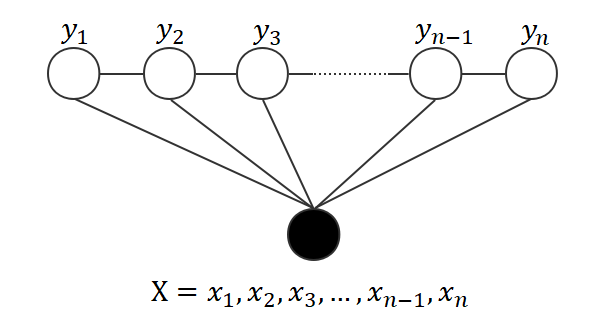
\includegraphics[width=0.9\textwidth]{./figure/线性链条件随机场.jpg}
\caption{线性链条件随机场}
\label{lab:1}
\end{minipage}
\end{figure}

条件随机场实际上是定义在时序数据上的对数线性模型,具有表达长距离依赖性和交叠性特征的能力,能够较好地解决标注偏置等问题。

\section{词向量}
分布式词嵌入是自然语言处理中一组语言建和特征学习技术的总称。将词汇表中的单词或短语映射成预定好维数的实数向。从数学空间映射的角度来看,这个过程是将一个维数等于不同词语数量的空间映射到一个连续的低维向量空间。生成这样映射的方法有神经网络、基于词共现的维数约减等方法。将词语等文本信息通过这样的分布式表现形式作为嵌入,这样的方法已经被证明可以提高自然语言处理任务的效果。

将文本表达成计算机可以理解的形式是自然语言处理任务的第一步。最早最朴素的表示方法是独热表示法(One-hot Representation),即用向量的每一维表示词库中的一个词。例如:

“中国”表示为[1,0,0,0,……,0,0]

“美国”表示为[0,1,0,0,……,0,0]

显然向量的维数是词语的总数,这样的表示方法简单易于理解,但是浪费极大的空间,而且并不能表现出词语与词语之间的关联。将单词表示为较低维度的向量的技术起源于20世纪60年代信息检索向量空间模型的发展。使用奇异值分解减少维度的数量,然后在20世纪80年代后起引入了潜在语义分析(LSA),2000年Bengio等\cite{Bengio}在一些列论文中提出了神经概率语言模型,通过对学习单词的分布式表示来降低上下文中单词表示的高维性。该领域在2010年后逐渐发展真正成为一种热门的方法,一个重要的原因是在那时向量训练的质量和速度方面取得了重要的进展。许多研究组开始在单词嵌入上投入更多经历。2013年,由Tomas Mikolov领导的谷歌团队创造了Word2Vec这样一个单词嵌入工具包,相较于之前的方法,该模型可以更快地训练出向量空间模型。现今大多说新的单词嵌入技术都是基于神经网络架构,而不是传统的n-gram模型和无监督学习。

训练word2vec有两种经典的模式CBOW和Skip-gram模型。

(1)CBOW

CBOW模型训练的方法是通当前词语的上下文词语来预测该词的向量。因而CBOW(Continuous Bag-of-Words)的输入是当前词上下文的词向量,输出就是当前词的词向量。比如下面这句话,“国家主席/习近平/在/进博会/上/宣布/设立/科创板/,并/于/板块/内/进行/注册制/试点/。”我们上下文窗口取值为6的话,特定词为“科创板”,即我们需要求出“科创板”的词向量,前后各有6个词共12个,这12个词是CBOW模型的输入,在最基本的CBOW模型中,采用的是词袋模式,即这12个词的权重一致,并不考虑每个词和目标词的距离。

\begin{figure}[h]
\centering
\begin{minipage}[t]{0.5\textwidth}
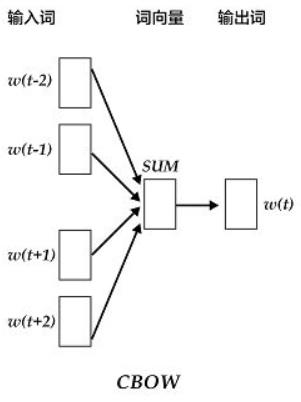
\includegraphics[width=0.9\textwidth]{./figure/CBOW模型.jpg}
\caption{CBOW模型}
\label{lab:1}
\end{minipage}
\end{figure}

CBOW模型的网络结构如图所示,在CBOW模型中输入的是12个词向量,输出的是所有词的softmax概率,损失函数是期望u内联网本特定词对应的softmax概率最大。对应的CBOW模型输入层是12个神经元,输出层的个数和词汇表的总大小一致,有词汇表大小个神经元。隐藏层的神经元个数可以自行设定,对于神经网络的求解通过经典的反向传播算法求解,迭代完所有语料便可以求解出所有词汇表中的词向量。

(2)Skip-gram

\begin{figure}[h]
\centering
\begin{minipage}[t]{0.5\textwidth}
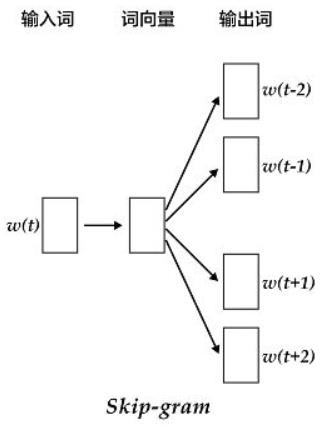
\includegraphics[width=0.9\textwidth]{./figure/Skip-gram模型.jpg}
\caption{Skip-gram模型}
\label{lab:1}
\end{minipage}
\end{figure}

Skip-gram模型与CBOW模型相反,Skip-gram是输入特定的一个词向量,反而输出的是上下文的词向量,例如上文的例子的话输出的就是上下文12个词的词向量,同样用反向传播算法,求出概率排前12的softmax该列车对应的神经元对应的词即为所求。

word2vec有许多重要的参数直接决定了训练的效果。上下文窗口决定了给订单词前后包含多少个单词作为上下文单词,在原始的word2vec模型中窗口内各个单词的权重一直,也有一些研究加权词向量的训练方法\cite{myh}来提高词向量的质量。维度也是影响词向量的因素之一,研究表明嵌入词的质量随着维数的增加而提高,但达到某一点后,边际效益将减少\cite{Mikolov}。
在word2vec模型实际运作中,为了解决词汇表太大,训练时间太长的问题,哈会使用霍夫曼树等方法优化训练过程,节省训练的时间。半采样也是实际word2vec训练中常用的优化方法,因为高频词通常提供的信息很少,频率高于设定阈值的单词会被降采样来提高训练的速度和质量。

\section{循环神经网络}

\subsection{循环神经网络概述}

深度学习是基于学习数据表示的更广泛机器学习方法的一种,深度神经网络是深度学习中最重要,应用最广的模型。深度神经网络体系结构已应用与计算机视觉、语音识别、自然语言处理、音频识别、机器翻译、生物信息学、药物设计、医学图像分析等领域。递归神经网络是一类人工神经网络,这类网络善于 预测未来。常用于分析时间序列数据,例如股票价格;在自动驾驶中可以预测汽车的行驶轨迹,避免事故。总的来说这样的网络可以输入文本、句子、语音等,使用到机器翻译、语音识别、语义分析等任务中。

\begin{figure}[h]
\centering
\begin{minipage}[t]{\textwidth}
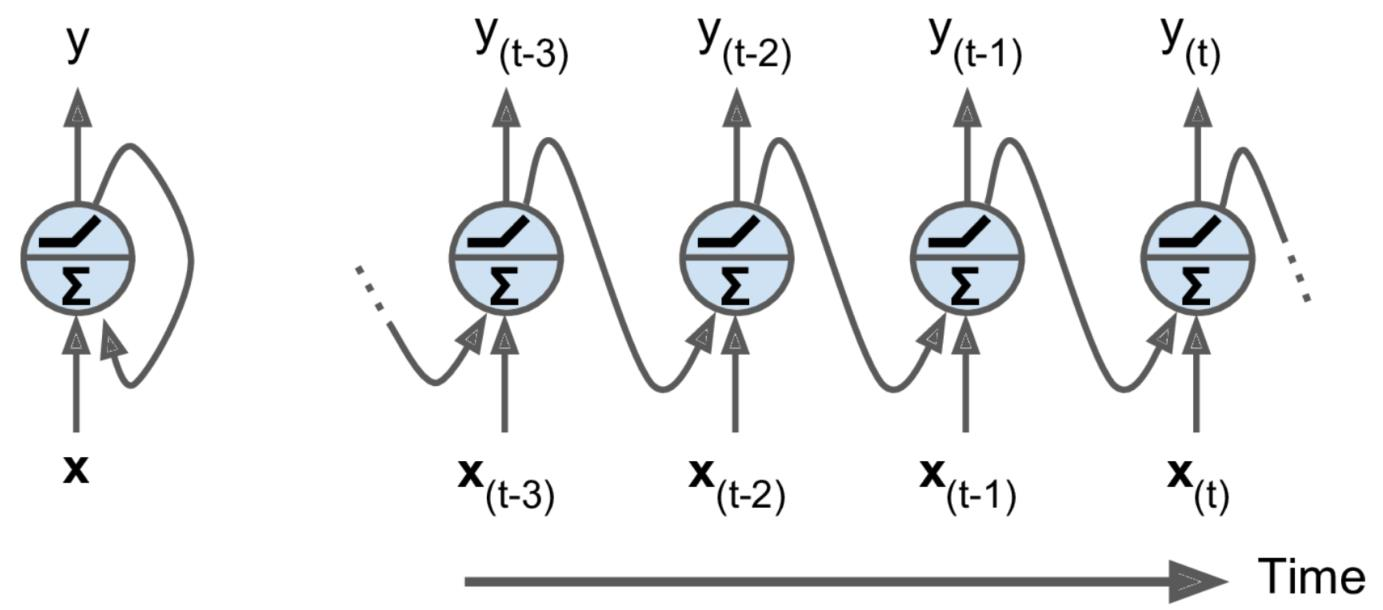
\includegraphics[width=0.9\textwidth,height=5.0cm]{./figure/simple_rnn.jpg}
\caption{简单的RNN模型}
\label{lab:1}
\end{minipage}
\end{figure}

\begin{figure}[h]
\centering
\begin{minipage}[t]{\textwidth}
\includegraphics[width=0.9\textwidth,height=5.0cm]{./figure/RNN层.jpg}
\caption{一个RNN层和展开结构}
\label{lab:1}
\end{minipage}
\end{figure}

不同于前馈神经网络,循环神经网络激活方向不仅仅只向一个方向流动。最简单的RNN,只由一个神经元接受输入产生输出,然后将输出发回自身,如图2-4所示。每个时间步骤t,每个神经都从上个时间步骤$y _ { ( t - 1 ) }$接收输入向量x和输出向量,一层RNN神经元如图所示。

由于在时间步骤t时刻循环回去的信息是上一个时刻的信息,这种网络结构使得输入可以是以前的时间步骤,因而在某种意义上RNN是一种具有“记忆”的神经网络结构。单个盛景园在时间步骤间保持某种状态,成为记忆单元。单个循环神经元或是一层循环神经元是一个基本结构,有更多复杂的网络结构是以这样的基本结构堆叠出来的。RNN可以同时接受一些列输入并同时产生一系列输出,如图所示。这样的类型的网络在处理序列数据上有着非常好的表现,可以用于预测时间序列等任务。

\subsection{长短期记忆网络}

长短期记忆网络(LSTM)细胞是由Sepp Hochreit和Jurgen Schmidhuber于1997年提出的\cite{Hochreit},并在多个领域任务上创造了记录。在语音识别技术、连续手写识别领域都曾创造当时的最佳纪录。2014年后,在深度神经网络模型中收到了广泛的应用,如果将LSTM单元视为一个黑盒,那么它可以非常像一个基本单元,并且性能会更好,训练收敛也更加容易,并且这种结构可以检测数据中的中长期依赖性。
如果不看LSTM单元内的结构的话,LSTM单元看起来和一个普通单元一样,知识它的状态被分成两个向量:${ h } _ { ( t ) }$和$ { c } _ { ( t ) }$,可以将${ h } _ { ( t ) }$看做短期状态,${ c } _ { ( t ) }$看作长期状态。LSTM单元的结构如图所示。



\begin{figure}[h]
\centering
\begin{minipage}[t]{\textwidth}
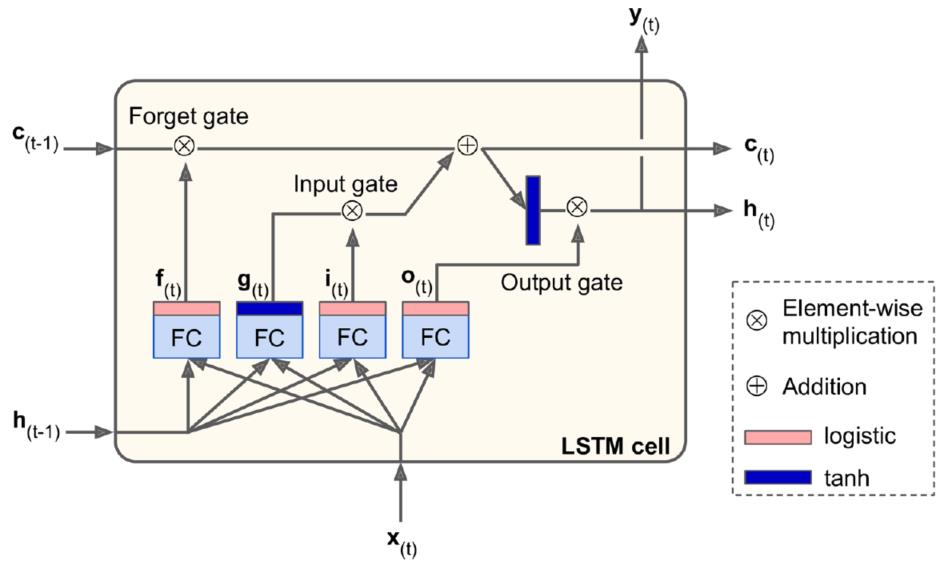
\includegraphics[width=1.0\textwidth,height=7.0cm]{./figure/LSTM.jpg}
\caption{LSTM单元}
\label{lab:1}
\end{minipage}
\end{figure}

长短时记忆网络的思路很简单,相较原始RNN结构比,原始RNN隐藏层只有一个状态h,这个状态对短期的输入敏感对长期的输入不敏感。因而LSTM单元中,增加一个状态c,用这个状态来保存长期状态。LSTM有能力向单元状态中添加或是一处信息,通过结构来管理,这种结构称为门限。LSTM关键思想是让网络可以学习长期状态下选择性地存储的内容、丢弃内容以及从中读取内容。当长期状态${ c } _ { ( t ) }$从左向右穿越网络时,可以看到数据流首先通过一个起始门,丢弃一些记忆,然后通过加法运算(添加由输入门选择的记忆)添加一些新的内存,最终${ c } _ { ( t ) }$不做更多的转换被直接发送出去。因而在这个模型中,在每一个时间步中,一些记忆被丢弃,一些记忆被添加进来。除此以外,${ h } _ { ( t ) }$在执行了第二步操作后,对长期状态进行复制并通过tanh函数传递,然后通过输出门对结果进行过滤。这就产生了短期状态(相当于在这一个单元步骤中的输出)。

简要而言,一个LSTM单元在输入门,可以学习去识别一个重要的输入,并将输入存储在长期状态中。只要没有被遗忘门作用的话,这个状态会一直被保存,直到需要的时候抽取走这个状态。这就解释了为何LSTM模型可以成功的原因,LSTM模型的特点就是捕获长期模式,因而在长时间录音、文本、音频等任务上有很好的发挥。

LSTM的训练方法也可以采用梯度下降法来最小化训练误差,一个经典的方法是应用时序性倒传递算法,这种算法依据错误修改每次的权重。用梯度下降法训练循环神经网络(RNN)时会产生一个严重的问题,误差梯度随时间长度成指数级别增长式得消实。而当设置成LSTM单元时,误差可以被重新抽取倒回计算,从输出端回到输入端,再重新经过每一个门限,直到数值被与之过滤掉。因此含有LSTM的单元的RNN可以被有效训练并记住长时间的信息。

\section{主题模型技术}

\subsection{潜语义分析}

潜语义分析(LSA)是一种对文档主题进行建模的方法,通过产生一组与文档和词语相关的概念来分析文档与其包含的词语之间的关系。LSA假设意义相近的单词出现在相似的文本片段中。通过语料集构建包含每个段落的词语的矩阵(行代表一个唯一的单词,列代表每个文档或段落),使用奇异值分解(SVD)技术来减少行数,同事可以保持列之间的相似性结构。取任意两行形成的两个向量之间的角度余弦来比较单词。接近1的值表示非常相似的单词,而接近0的值表示非常不同的单词。用任意两列向量之间角度的余弦来比较文档,接近1的值表示非常相似的文档,而接近0的值表示非常不同的文档。

\begin{figure}[h]
\centering
\begin{minipage}[t]{\textwidth}
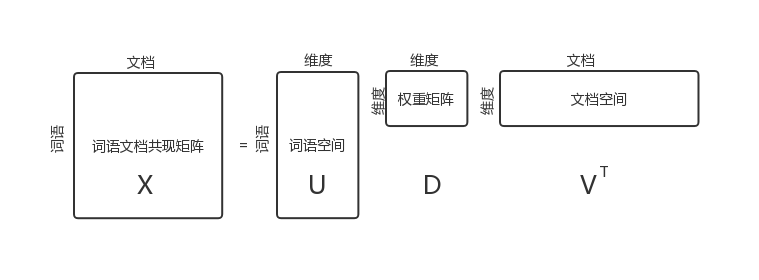
\includegraphics[width=1.0\textwidth,height=5.0cm]{./figure/LSA.jpg}
\caption{LSA模型}
\label{lab:1}
\end{minipage}
\end{figure}

$$X = U D V ^ { T }$$

LSA模型如上图所示,矩阵U中的每一行表示每个词在每个词类(主题)的值,每一列表示语义相近的词类,每行中的值表示每个词语在这个语义类中的重要程度。LSA可以刻画同义词,因为词语相近的词对应着相同或相似的主题,SVD的降维方法也可以去除部分噪声,使得特征鲁棒性更好。但是LSA无法处理一词多义的问题,LSA将每个词映射到了潜语义空间中的一个点,即一个词对应的多个含义没有被区分。并且LSA的概率模型,是以文档和词的分布服从联合正态分布为前提假设的,但这个假设往往准确性不高。

\subsection{概率潜语义分析}

概率潜语义分析(PLSA)是根据观察到的变量与某些隐藏变量的相似性从而得出它们的低维表示,这种技术是潜语义分析技术的一个改进版本。与LSA是利用线性代数方法进行降维不同的是,PLSA是基于估计一个概率模型参数达到降维效果。PLSA模型将文档中的词看作来自混合模型的采样,假设每个词来自一个主题,同一个文档中不同词可能来自不同的主题。再将文档表示为多个主题的混合,每个主题具有不同的概率,每个主题又由多个词构成。

\begin{figure}[h]
\centering
\begin{minipage}[t]{\textwidth}
\includegraphics[width=0.8\textwidth,height=4.0cm]{./figure/PLSA.jpg}
\caption{PLSA模型}
\label{lab:1}
\end{minipage}
\end{figure}

$$P ( w , d ) = \sum _ { c } P ( c ) P ( d | c ) P ( w | c ) = P ( d ) \sum _ { c } P ( c | d ) P ( w | c )$$

上式中$P ( d )$表示从文档集合选择文档d的概率,$P ( c )$表示选择主题c的概率,主题个数是PLSA模型中的超参数需要提前设定,这里主题c是隐变量。在已知文档$P ( d )$和其对应词表w后,对主题进行推断。即求解

$$p ( c | d , w ) = \frac { P ( c ) P ( d | c ) P ( w | c ) } { \sum _ { c ^ { \prime } \in C } P \left( c ^ { \prime } \right) P ( d | c ^ { \prime } ) P ( w | c ^ { \prime } ) }$$

PLSA对参数的求解通过EM算法进行学习。PLSA像比如LSA可以较好的解决一词多义的问题,相比于LSA,PLSA使用多项式分布在真实数据上表现来说优于LSA。然而PLSA的训练常常会遇到过拟合的问题,即训练出的数据效果在训练集上很好但是在其他语料上的表现差异较大。

\subsection{隐狄利克雷分配模型}

隐狄利克雷分配模型(LDA)是有PLSA的基础上发展而来。LDA是一个生成式的统计模型,假定每个文档都是少量主题的混合体,并且每个单词的出现都归因于文档中的某个主题。

\begin{figure}[h]
\centering
\begin{minipage}[t]{\textwidth}
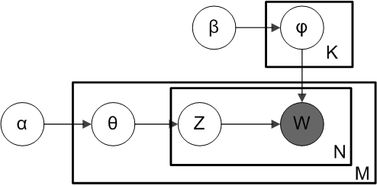
\includegraphics[width=0.8\textwidth,height=5.0cm]{./figure/lda.jpg}
\caption{LDA模型}
\label{lab:1}
\end{minipage}
\end{figure}

PLSA模型和LDA模型在建立文档和主题间的概率模型和建立主题与词的概率模型时都采用了多项式分布,为了计算的简便性并且让先验更有意义,LDA在PLSA的基础上做了改进,选取了多项式分布的共轭先验分布狄利克雷分布作为概率分布的选择。如图2-9,Z是主题,$\theta$是决定文档主题的概率分布参数,$\alpha$是决定文档对主题的概率分布参数$\theta$的超参数。W是特定的单词,$\varphi$是词语对主题的概率分布的参数,$\beta$是决定词语对主题的概率分布参数$\varphi$的超参数。形式化来说:

$$\theta _ { i } \sim \operatorname { Dir } ( \alpha ), i \in \{ 1 , \ldots , M \}$$
$$\varphi _ { k } \sim \operatorname { Dir } ( \beta ), k \in \{ 1 , \ldots , K \}$$
$$z _ { i , j } \sim \text { Multinomial } \left( \theta _ { i } \right), i \in \{ 1 , \ldots , M \},j \in \left\{ 1 , \ldots , N _ { i } \right\}$$
$$w _ { i , j } \sim \text { Multinomial } \left( \varphi _ { z _ { i , j } } \right), i \in \{ 1 , \ldots , M \},j \in \left\{ 1 , \ldots , N _ { i } \right\} $$

LDA模型求解是一个较为复杂的最优化问题,精确求解较为困难,一般采用近似求解方法。主要的求解方式是采用吉布斯采样算法、基于变分的EM算法和基于期望推进的方法。最主流的方法是吉布斯采样方法,这种方法基于马尔科夫链的蒙特卡洛方法。这种方法收敛较快、容易并行化,效果也不错,因为被广泛使用。LDA模型在缺少海量数据的情况下表现明显超出PLSA模型,有较强的抗过拟合性,成为一种经典的主题模型方法。

\section{本章小结}

本文介绍了论文研究所涉及的模型与技术。先从命名实体建模方法开始介绍,引出命名实体的标注方法;接着介绍了条件随机场这种解决序列标注的经典模型;后文通过介绍词向量和循环神经网络介绍当下较为先进的命名实体识别问题的关键技术;最后介绍了本文工作中使用的主题模型方法。


\chapter{改进的中文字符级特征表示方法}

\section{引言}

命名实体识别任务是自然语言处理任务中的重要任务之一。命名实体指一个词语或者一个短语明确指称一个标识的实体,一般有人名、机构名、地名等。命名实体识别是将文本中的命名实体定位并分类为预定义的实体类别的过程。目前解决命名实体识别的成熟方法是将命名实体问题建模成序列标注问题,首先将词语分布式表示,通过深度神经网络训练,最终通过条件随机场层输出。本文工作的基础模型是字符向量嵌入-BiLSTM-CRF模型进行命名实体识别,以该模型为基础解决中文复杂命名实体识别问题。

相比于英文命名实体识别,中文命名实体识别要困难的多,因为英文天然的空格隔开词语,不同词性的词语词缀词根也不同,直接训练词向量做为特征的分布式表示就能达到不错的效果,但是中文词语间没有间隔,一词多义,在特征表示上相交英文来说效果不够好。

本章的工作就是面向中文文本的特征表示,针对中文命名实体问题改进中文字符级特征表示方法。本章的主要创新点是:(1)针对字符向量一字多义难以区分的问题,提出基于位置信息丰富单个字符的向量优化方法;(2)针对字符向量训练时受制与上下文窗口大小的限制,字符向量信息量少,提出基于主题信息的字符向量构造方法。

本章章节内容安排如下:3.2节介绍命名实体分布式特征表示的相关理论与工作;3.3节介绍本章工作的基础模型基于字符向量的BiLSTM-CRF命名实体识别模型;3.4节介绍面向位置信息的字符向量优化方法;3.5介绍面向主题信息的字符向量构造方法;3.6节描述实验方法及实验结果和分析;3.7节是本章小结。

\section{相关理论与工作}

本节介绍命名实体识别领域在特征表示方面的工作,这些工作是本文的研究基础,也是本文工作的理论支持。深度学习这种能力强大的模型近年来在多个领域取得了进展和突破,在命名实体领域也有不错的表现。深度神经网络一个很大的优点就是该模型可以在训练过程中自动寻找数据的特征,因而采用深度学习完成命名实体识别任务的第一个任务环节就是要将文本进行分布式表示。

在英文文本特征表示方法上,近年有许多启发性的研究成果。\cite{Strubell}提出一种基于迭代扩张卷积神经网络(ID-CNN)的标记方案,通过skip-ngram对SENNA语料库进行100维嵌入式训练。\cite{JLi}不仅仅局限在单词的维度,而是将字符拆解为词缀词根进行分布式表示。\cite{Kuru}提出一个字符级的命名实体识别模型,并给出一个字符级的标注标签,该模型将一个句子看作是一个字母的序列,之后用LSTM抽取字符级别的表示,抽取命名实体。混合单词信息、字符信息、词缀词根信息、单词主题信息的模型\cite{Strubell}\cite{Wei}\cite{Jansson}在命名实体识别模型上也有一定的功效。近期还有Devlin等\cite{Devlin}提出一个新的语言表示模型BERT,BERT基于所有层中的左、右语境进行联合调整,来预训练深层双向表征,在很多任务上达到了很好的效果。

在中文文本特征表示方法上,Yue等\cite{Yue}等提出了一个词格模型来解决中文命名实体识别问题,不仅使用每个汉字字符的信息,再加上所有可能构成的所有单词的信息,这样的模型有效地减少了分词错误,对词典构造有一定依赖。Zhao等\cite{Zhao}实现了一个高速LSTM-CRF模型,在高速层自动选择与当前字符更相关的单词,达到了与注意力机制相似的效果。林泽斐等\cite{lzf}利用上下文信息对应的知识库知识,对于命名实体识别任务中的命名实体进行消歧。王超等\cite{Wang}利用LSTM中文分词技术优化分词模块,在中文微博命名实体识别上取得了较好的效果。

\section{CharEmbedding-BiLSTM-CRF中文命名实体识别模型}

\subsection{模型比较与优势}
经过大量的文献综述和前沿方法总结,我们可以得出结论,目前主流成熟的深度学习中文命名实体识别方法大致流程是:(1)字词的分布式表示(2)深度学习网络有监督训练模型(3)对序列中的每个字词进行标签标注。本论文使用的基准模型是CharEmbedding-BiLSTM-CRF命名实体模型,选择该基准模型是因为其有着建模合理,效果优良,优化潜力大等优点,理由如下:

(1)字符嵌入方面。基于词语的嵌入方式的缺点是,中文词语切割是基于字典的,这样的分词技术一旦出现错误则后续的命名实体任务很难成功,因而基于词语的嵌入方式模型容量较低。对于各种基于分词的中文命名实体对于解决地名识别、组合型组织名(例如“中国国家男子足球队”)效果较好,但是对于人名、企业名等不是由词语构成的命名实体效果不好,因为这类命名实体组成方式和普通构词方式差异较大。因而选取直接字符嵌入作为基模型研究。

(2)神经网络方面。传统的前馈神经网络(例如CNN)在分类任务上略有优势,然而对于信息序列来说,信息见彼此有着复杂的时间关联性,更重要的是对于命名实体识别任务来说信息长度各不相同,前馈神经网络建模困难,表现往往不好。因而对于序列任务反馈神经网络(即循环神经网络)将是优先的选择。而LSTM模型是RNN的一个特例,在善于对序列问题建模的同时,还有着易于求解,能够长期保存重要信息。而双向长短时记忆网络(BiLSTM)是LSTM模型的一个改进版本,传统的RNN输入是上文,输出是下文,根据上文推出下文,双向RNN同样利用反向信息,让模型从两个方向学习,这个概念也符合中文自然语言的构词遣句的思想。BiLSTM便是LSTM的双向版本,实验证明BiLSTM往往比LSTM有着更好的表现\cite{Graves},特别实在序列标注模型上\cite{Huang}可以同时学习过去的序列和未来的序列有着更好的效果。因而神经网络模块本文选择BiLSTM模型。

(3)序列标注模型方面。最常用的方法是条件随机场(CRF)和接全连接层用softmax激活。CRF将输出层面的关联性分离出来,在预测标签时可以充分考虑上下文关联,更重要的是CRF的求解维特比算法是利用动态规划的方法求出概率最大的路径,这与命名实体识别的任务契合的更好。因为本文序列标注上选择CRF模型。

\subsection{模型流程与实现}

(1)字向量训练

中文字符向量的训练与词向量的训练相似,对于中文语料集首先去除非字符,按每个字符作为一个输入按空格隔开。本文训练语料采用的是人民日报2014数据集,窗口大小设置为5,采用Skip-gram模式训练字向量。经统计不同字符有4000左右,按经验设置隐层神经元个数为100,即训练100维度的字向量。

\begin{figure}[h]
\centering
\begin{minipage}[t]{\textwidth}
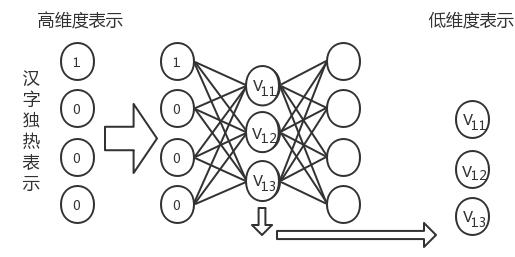
\includegraphics[width=0.5\textwidth,height=5.0cm]{./figure/char2vec.jpg}
\caption{中文字符向量表示}
\label{lab:1}
\end{minipage}
\end{figure}

经过多轮迭代训练,训练出中文字符向量。这里举例“全”、“国”、“政”、“协”、“会”、“议”六个字向量,在全部词典中找出与该字向量最相近的字向量,以观测字向量训练的效果,结果如表3-1所示。

\begin{table}[H]
\centering
\begin{tabular}{cccccc} %l(left)居左显示 r(right)居右显示 c居中显示
\hline 
全& 国& 教& 育& 会& 议\\
\hline  
整 0.5757& 华 0.5501& 堂 0.6539& 培 0.6382&协 0.6194&审 0.5820\\
排 0.5665& 兰 0.5284& 宗 0.6387& 教 0.6091&届 0.5958&谘 0.5698\\
障 0.5405& 洲 0.4830& 徒 0.6241& 体 0.5926&参 0.5499&选 0.5566\\
中 0.5101& 暨 0.4752& 皈 0.6185& 训 0.5667&员 0.5341&协 0.5540\\
防 0.5080& 侨 0.4752& 育 0.6091& 课 0.5374&暨 0.5175&党 0.5508\\
第 0.4943& 央 0.4733& 督 0.6034& 养 0.5369&动 0.5121&遴 0.5474\\
并 0.4930& 联 0.4723& 仰 0.6017& 健 0.5367&团 0.5109&席 0.5432\\
会 0.4913& 盟 0.4606& 圣 0.5998& 学 0.5275&办 0.5061&宪 0.5429\\
\hline 
\end{tabular}
\caption{字向量训练效果}
\end{table}



word2vec这样的模型不仅将词汇用我们设定的维度分布式表达,同时也能够保留字与字之间的语义联系,很多文献\cite{Yoon}与工作表明这样分布式的表现对后续神经网络处理自然语言问题有着很好的效果。选取部分100维字向量用主成分分析法(PCA)降维至两个维度,在可视化的二维平面作图(见图3-2),可见语义相近的字向量降维后的坐标相互靠近,语义无关的字向量距离较远,说明字向量的训练达到了一个较好的效果。

\begin{figure}[H]
\centering
\begin{minipage}[t]{\textwidth}
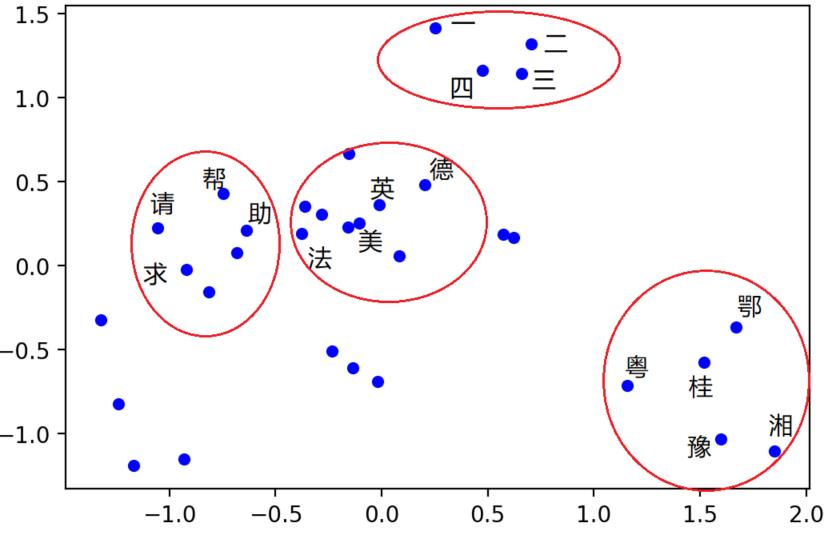
\includegraphics[width=0.8\textwidth,height=7.5cm]{./figure/字向量降维.jpg}
\caption{训练出的字向量降维效果图}
\label{lab:1}
\end{minipage}
\end{figure}



(2)神经网络构建

神经网络模型选取双向长短时记忆网络(Bidirectional LSTM Networks),传统的RNN模型在训练中会遇到梯度爆炸和梯度消失等难以求解的问题。所谓的梯度消失和梯度爆炸问题都是在通过反向传播训练计算时,梯度倾向于在每一时刻递增或者递减,经过一段时间后梯度就会发散到上限或是衰减到零。对于梯度发散的问题一般可以通过设定阈值使得梯度不能超过一个给定值来解决,但是对于梯度消失问题,简单的RNN模型就无法解决。在命名实体识别这样的序列标注问题中,梯度消失就表现为网络难以联接到远处的信息能力。如图3-3,简单的RNN模型对于传递较远的信息在训练时往往受梯度消失的影响而消失。

\begin{figure}[H]
\centering
\begin{minipage}[t]{\textwidth}
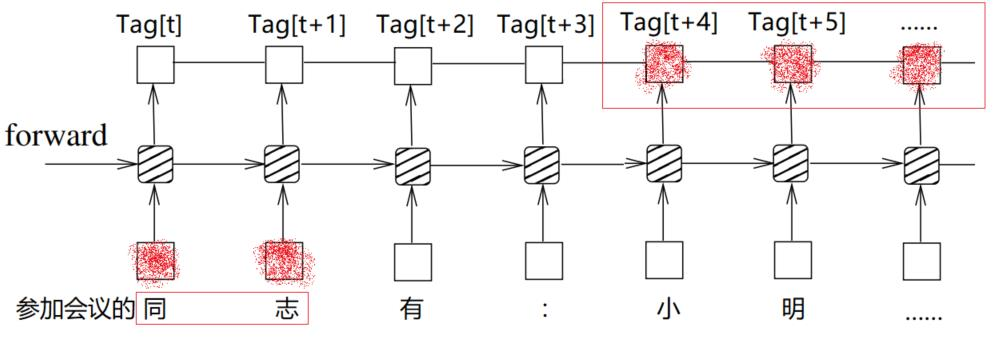
\includegraphics[width=0.8\textwidth,height=4cm]{./figure/命名实体识别长期信息.jpg}
\caption{命名实体识别中的长期信息}
\label{lab:1}
\end{minipage}
\end{figure}


除此以外,命名实体问题与前向信息和后向信息都有很大的关联。例如“美国总统特朗普”、“百度(中国)有限公司”、“钱学森院士等参加座谈”,通过这些语言片段,我们可以发现我们人类识别出人名、地名、组织名的过程中,往往是借助该实体前文的信息和后文的信息。正因如此,对于命名实体识别问题,构建向前和向后两个循环神经网络框架是一个更优的选择。如图所示命名实体识别问题中,前向信息和后向信息对于命名实体的识别都有着相当大的贡献。

\begin{figure}[h]
\centering
\begin{minipage}[t]{\textwidth}
\includegraphics[width=0.8\textwidth,height=4cm]{./figure/BiLSTM与NER.jpg}
\caption{双向LSTM示意图}
\label{lab:1}
\end{minipage}
\end{figure}

(3)条件随机场与序列标注

条件随机场模型(CRF)相较于传统分类模型而言,不仅仅关注个体标签的分类,还非常关注句子级别的信息,近些年的工作表明CRF模型在序列标注问题上有着很高的准确率。CRF层可以通过训练语料学习得到一些基于全局的约束信息,比如句子中识别出的实体标签的起始应当是“B-”而不是“I-”;不同类的标签不会相互连接,识别出的人名、地名、组织名标签不会混搭,从而能够识别出准确的命名实体。整体CharEmbedding-LSTM-CRF命名实体识别模型框架如图3-5。

\begin{figure}[ht]
\centering
\begin{minipage}[t]{\textwidth}
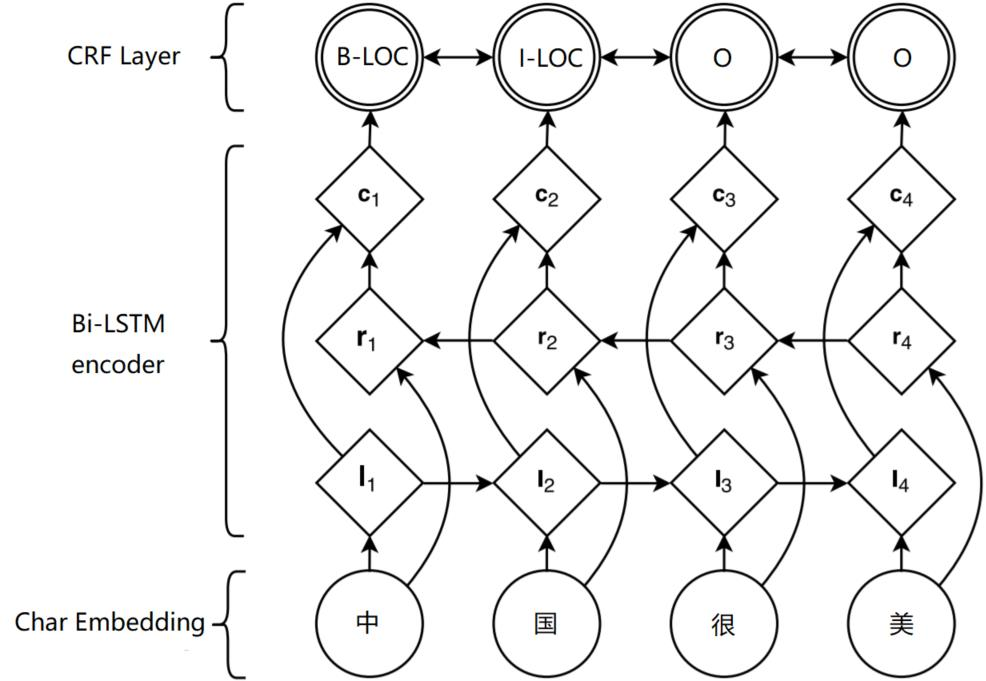
\includegraphics[width=0.8\textwidth,height=8cm]{./figure/CE-LSTM-CRF.jpg}
\caption{CharEmbedding-BiLSTM-CRF模型}
\label{lab:1}
\end{minipage}
\end{figure}

设我们输入的序列是$X=\left(x_{1}, x_{2}, \ldots, x_{n}\right)$,经过分布式表示和BiLSTM模块后输出的概率矩阵为$P_{n * k}$,其中k是标签的个数(例如在BIO标签系统内识别人名地名组织名,标签的个数为7).$P_{i, j}$指$x_{i}$被标记为第j个标签的概率。$A_{i, j}$代表概率转移矩阵中第i个标签转移到第j个标签的概率。

对于将要输出的标签序列$y=\left(y_{1}, y_{2}, \ldots, y_{n}\right)$,定义如下路径得分公式:

\begin{equation}
S(X, y)=\sum_{i=0}^{n} A_{y_{i}, y_{i+1}}+\sum_{i=0}^{n} P_{i, y_{i}} 
\end{equation}

\begin{equation}
y^{*}=\operatorname{argmax} S(X, y)
\end{equation}

CRF模型通过对输出标签二元组进行建模,使用动态规划算法找出得分最高的路径$y^{*}$作为最优路径进行序列标注。

在神经网络模型训练的过程中,每轮训练用当前batch作为测试样例,通过网络模型得出本轮次预测的标签,在一个条件随机场里计算标签序列的对数似然值,以此作为神经网络的损失函数。通过误差逆传播算法,用一轮轮训练数据去优化神经网络的参数,直到模型参数稳定,训练误差长时间不再缩小为止。这样就将整个模型训练完毕,通过该模型可以对中文文本进行命名实体识别工作。



\section{基于位置信息的中文字符向量优化方法}

将文本信息进行分布式表示是深度神经网络自动抽取特征,处理自然语言问题的关键步骤。这一过程将计算机程序不容易理解的字符串,转化为分布式的形式,便于神经网络去拟合复杂度更高的函数。使用word2vec训练词向量这种方法将文本的分布式表示与字词间的含义联系起来,消除了词语鸿沟的现象。使用预训练好的词向量作为深度学习处理自然语言问题已经成为一个经典成熟的方法,很多工作证明使用预先训练好的词向量与随机嵌入相比,整个神经网络收敛速度更快;训练好的模型在准确度和召回度上都有较大的提升;特别是在数据量较小的情况下使用word2vec的方法优势更加明显。

然而当前在中文命名实体识别任务中,特征的分布式表示还有很多待解决的问题。由于中文和英文不同,没有空格间隔开词语,而单字对语义表达的能力不强,同样的中文词语可能意义不同词性不同,同样的汉字含义词性更是千差万别。为了解决中文命名实体识别问题中的特征分布式表示问题,多种解决方向也在被研究者们不断地探索:一类工作是在分布式表示时加入中文分词词典信息,比如中文分词后进行词向量的嵌入,这类方法的局限性是识别结果较依赖于构建的中文词典,而命名实体识别任务中较为关注的人名、组织名这样的实体他们的命名往往与分词技术相抵触,这类实体的命名往往碎片性、象征性、随机性更强和组词关系较小。例如“邓小平常说教育要从娃娃抓起。”这句话,分词时很容易发生分出“平常”的错误从而导致人名识别的失败,中文词典不可能收录无穷尽的人名组织名,这样的目标也与命名实体的目的相违背。另一类工作是寻找中文字符更小的粒度,就像英文工作中将单词粒度细分为词根词缀等一样,将中文汉字按偏旁部首继续细分,从更小的粒度寻找更细节的特征。汉字和英文单词发展有所区别,汉字起源于象形文字,每个偏旁部首带有一定的含义,在演化的过程中,汉字被不断简化,同音字合并,一字多音等现象十分频繁,这些导致偏旁部首的信息也更加复杂。这类方法对于寻找更细节的特征有助益,但对于解决命名实体识别问题中一字多义的问题还是较为乏力。

根据文献综述和对CharEmbedding-LSTM-CRF模型的实验结果分析,可以发现影响命名实体识别准确度召回度的很重要原因就是一字多义问题。中文常用汉字只有3500左右,而英文常用单词有30000个左右,从这个角度来看,在同样的语义空间内英文单词的词向量信息是源多于中文字符向量的,也就是说汉字一字多义、一字多性的现象十分普遍。

\begin{figure}[ht]
\centering
\begin{minipage}[t]{\textwidth}
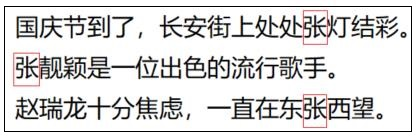
\includegraphics[width=0.55\textwidth,height=2.5cm]{./figure/一字多义.jpg}
\caption{一字多义、一字多性现象}
\label{lab:1}
\end{minipage}
\end{figure}

以上三句话中都含有“张”字,显然这三个“张”字的含义并不相同,词性也不同。然而在基本的中文字符向量嵌入方法中,这三个张字的字向量嵌入的完全一致,都是通过大量语料中“张”字出现时,窗口内的其余信息训练出的。如果能够尽可能的将不同含义的“张”字表示成不同的字向量,扩充整个字向量空间,使得整体字向量的表达能力更强,将字词鸿沟现象更好的解决,将会对后续使用字向量训练神经网络来解决命名实体识别问题带来相当可观的帮助。

通过上面的例子,我们同样可以得知,判断一个字符的含义如何,关键还是靠其周围的文字信息。能够在字向量的独立性和词向量的语义特征间取得一个平衡。因而本节提出一个字符向量基于位置信息的改进方法,具体过程如下:

对于一个句子输入$X=\left(x_{1}, x_{2}, x_{3},...,x_{t},... x_{n}\right)$,对应嵌入中文字符级$W=\left(w\left(x_{1}\right), w(n), \cdots w\left(x_{t}\right), \cdots x_{n}\right)$,这里w表示字符转换为字符向量的函数。X句子中第t个字符基于位置信息改进后的字向量表示为$w^{*}(x_{t})$,则其满足:
\begin{equation}
w^{*}\left(x_{t}\right)=s\left(x_{t}, x-\left\{x_{t}\right\}\right)
\end{equation}

即优化后的字符向量不仅与其本身的字符有关,还本句文本中其余的字符含义相关,为方便计算我们将训练的字符向量作为新模型中,本句其他字符的表示。为了统一形式,我们将原始$x_{t}$的向量提出,这样函数S=0时,字符向量即为初始的字符向量。

\begin{equation}
w^{*}\left(x_{t}\right)=S\left(w\left(x_{t}\right), w\left(x_{1}\right), w\left(x_{2}\right), \ldots, w\left(x_{t-1}\right), w\left(x_{t+1}\right), \ldots, w\left(x_{n}\right)\right)
\end{equation}

\begin{equation}
w^{*}\left(x_{t}\right)=w\left(x_{t}\right)+S\left( w\left(x_{1}\right), w\left(x_{2}\right), \ldots, w\left(x_{t-1}\right), w\left(x_{t+1}\right), \ldots, w\left(x_{n}\right)\right)
\end{equation}

这里为了简化模型,本文将函数S建模成一个线性函数,也就是说新的字符向量是原本的字符向量加上周边原字符向量的加和。这样的模型有其合理性,比如说“理发”、“发财”、“出发”,同样的“发”字,原本模型中向量相同,在改进后的模型中,字向量受到周边信息的影响,而周边字向量越相似的其修正后的字向量也就越相近,这也与现实中的词义关联一致,这样的方法可解释性较强。

\begin{equation}
w^{*}\left(x_{t}\right)=\lambda \cdot w \mbox{;} w \mbox{指X句子原始字符向量的矩阵}
\end{equation}

对于模型参数的确定,基于计算方便和贴近现实的角度,我们这里对模型参数进行一些假设。首先是模型参数的值按$x_{t}$对称,也就是说假定基于位置信息的影响前后两个方向是相同的,这也符合汉字组词的常识。再者就是,按照信息传播的性质,传播的信息随着距离的增长,信息传递随之减弱。自然语言处理中经典的N-Gram模型也同样有类似的假设,即$x_{t}$前后k个字符的信息,而忽略更远的字符信息。

\begin{equation}
w^{*}\left(x_{t}\right)=\lambda_{k} w\left(x_{t-k}\right)+\ldots \lambda_{2}w\left(x_{t-2}\right)+\lambda_{1} w\left(x_{t-1}\right)+ w\left(x_{t}\right)+\lambda_{1} w\left(x_{t+1}\right)+\ldots+\lambda_{k} w\left(x_{t+k}\right)
\end{equation}

\begin{figure}[H]
\centering
\begin{minipage}[t]{\textwidth}
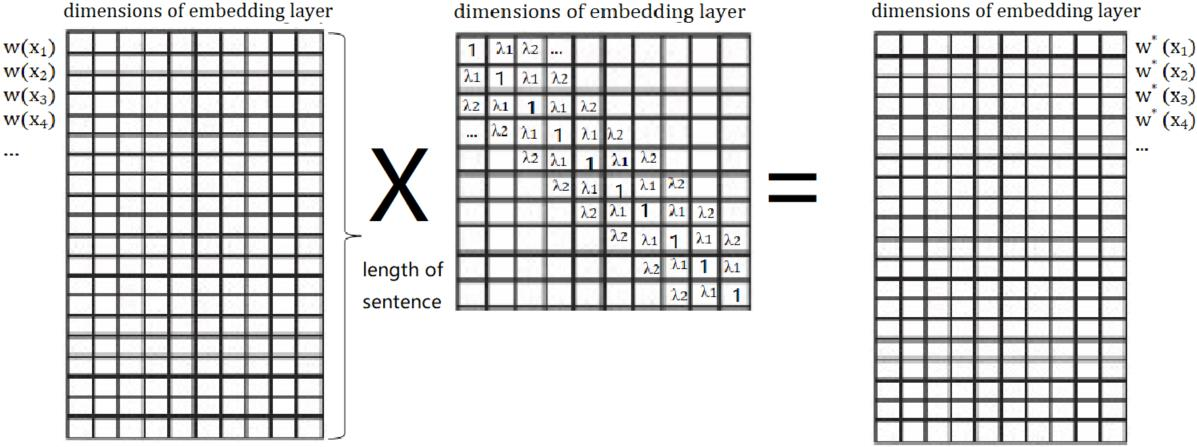
\includegraphics[width=1.04\textwidth,height=6.5cm]{./figure/基于位置信息变化.jpg}
\caption{基于位置信息优化初始字符向量}
\label{lab:1}
\end{minipage}
\end{figure}

本文对于该模型的参数求解的方法采用的是网格搜索法,具体实验过程与相关结果参见3.6节实验结果及分析。通过实验效果来看,这样的基于位置信息优化字符向量表示的方法提高了字符向量表示的效率。其他环节相同的情况下,在标准数据集上实验表明,这中优化方法提高了命名实体识别任务的准确率、召回率等指标。

\section{基于主题信息的中文字符向量构造方法}

在深度学习的分布式特征表示阶段,为了提高模型的效果,我们应该在特征表示阶段尽量加入足够多的信息以便于后续神经网络模型训练时自动对特征进行抽取,最终准确的对数据进行分类。在各类机器学习模型日臻成熟的今天,数据量的大小,对于数据特征的抽取和表示对整体机器学习模型的效果产生着越来越大的影响。

在word2vec训练词向量的过程中,是以一个窗口的区域来获得词与词之间的关系。对于CBOW方法是通过词语的上下文来预测当前词的向量,而在Skip-gram模型是按当前词的向量预测上下文的词向量。这样的学习关联主要还是基于窗口内的信息,而缺少对于全局信息的把握。总体而言word2vec对于短文本的训练学习有很好的语义表征效果,但是如果训练集是新闻正文这样的长文本的话,就会丧失对于同一篇文档属于同一个主题这样有用的信息。

如图3-8主题模型将原本的“词语-文档”按照隐含的“主题”概念,分解为“词语-主题”矩阵和“文档-主题”矩阵。“文档-主题”可以对文本进行聚类,而“词语-主题”矩阵也是一种词语的分布式表示。对于每一维隐含的主题,数值越高的越与该隐含主题相关性大,对于两个不同的词而言,主题向量越相近,他们背后的语义也越相近。有过一些工作是将主题信息引入到命名实体识别工作中:Jansson等\cite{Jansson}在英文命名实体任务中使用250个隐主题来加强词语的分布式表示;文献\cite{kang}在英文命名实体识别任务中联合卷积神经网络和词对主题模型对命名实体进行识别;文献\cite{gong}利用潜语义分析技术(LSA)对于条件随机场识别出的命名实体进行歧义消解。

\begin{figure}[H]
\centering
\begin{minipage}[t]{\textwidth}
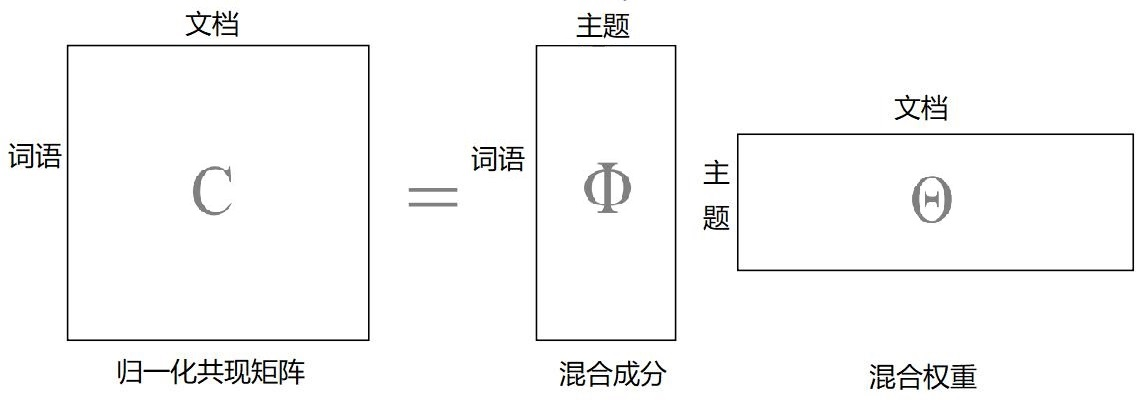
\includegraphics[width=0.8\textwidth,height=4cm]{./figure/主题模型.jpg}
\caption{主题模型}
\label{lab:1}
\end{minipage}
\end{figure}

比如说,一篇科技类的文章中涉及到“百度”、“阿里巴巴”、“腾讯”等,同时也出现了“李彦宏”、“马云”、“马化腾”等信息,这样一篇文档用主题模型训练,会让这些词的某个主题维度趋同于较大的概率。而只采用word2vec这样词向量的方法的话,训练的信息更多是公司之间、公司与对应老板间、老板与老板间的关系,而缺少了这些词之间交叉的关联,缺少了这些词背后潜在的主题相关度,这是由于word2vec模型窗口的大小不可能无限制扩大决定的。因此,如果将训练集中的全局主题信息加入,可以使得字符级的中文分布式向量容纳的信息更多更全,强化向量表示能力以达到提高整体CharEmbeddeing-LSTM-CRF命名实体识别模型效果的目的。主题模型这类非监督文本聚类方法假设一个文本(可以是一篇文章也可以是一个段落),隐含表达着一个主题,而这个主题可以由一个主题向量表示,主题向量越接近说明文本的相关性越强。不同于word2vec在大小为10左右的窗口内建模,主题模型基于篇章级别,只要在一篇文档内共现,主题模型都将计算词与词之间的联系。



基于前人工作和使用主题信息的合理性,本文将主题信息引入到中文字符级别的分布式表示中。采用隐狄利克雷分配模型(LDA),对字符级词语进行训练。将一个中文字符作为一个独立语义的词语,通过隐狄利克雷分配模型(LDA)训练模型。模型预先设置K个主题,每篇文档围绕这K个主题生成字。假设文档与主题符合多项式分布,字符与主题也符合多项式分布,而这两个多项式分布的参数符合具有先验参数的狄利克雷分布。主题模型的建模方法是,文档按概率选择主题向量中的一个主题,这个主题再按概率选择一个该主题下的字,这样的方法生成一整篇文档。我们的工作是需要训练这样的模型,得到字与主题之间的信息。


\begin{algorithm}[H]
    \caption{字符级主题向量训练算法}
    \label{alg1}
    \begin{algorithmic}[1]
        \STATE 输入:先验参数$\alpha$和$\beta$,主题数量$K$,语料集$D$
        \STATE 输出: 主题-字符参数矩阵$\phi$,文档-主题参数矩阵$\theta$
        \STATE 对文档中的所有中文字符进行遍历,为其随机分配一个主题,\\即 $z(m,n)=k \sim Mult(1/K )$,  
        \STATE 遍历文档,计算当前主题:\\
        $P(z_i=k|z_{\neg i}, w) = \frac {n_{k, \neg i}^t + \beta_t} { \sum_{t=1}^{V} n_{k,\neg i}^t + \beta_t} \cdot \frac {n_{m,\neg i}^k + \alpha_k} {\sum_{k=1}^{K} n_{m, \neg i}^k + \alpha_k }$
        \STATE 迭代完成后输出主题-字符参数矩阵$\Phi$,该矩阵即为不同的词语在不同主题下的概率情况
    \end{algorithmic}
\end{algorithm}

训练集采用腾讯新闻数据一万多篇不同类型的新闻文本,隐主题个数设为50,训练完成后,我们观察距离每个主题概率值最大的字符,效果如下:

\begin{table}[H]
\centering
\begin{tabular}{ccccccc} %l(left)居左显示 r(right)居右显示 c居中显示
\hline 
topic1& topic2& topic3& topic4& topic5& topic6&……\\
\hline  
教 0.032& 矿 0.175& 酒 0.019& 罪 0.015&狗 0.074&医 0.063&……\\
校 0.031& 煤 0.090& 驾 0.018& 刑 0.011&犬 0.029&疗 0.048&……\\
聘 0.023& 鹤 0.088& 斑 0.012& 贿 0.011&鼠 0.025&药 0.030&……\\
学 0.019& 岗 0.060& 肇 0.011& 犯 0.009&樟 0.024&蚁 0.015&……\\
詹 0.019& 井 0.055& 乳 0.011& 审 0.009&豚 0.018&诊 0.013&……\\
师 0.017& 炸 0.036& 车 0.011& 案 0.009&礁 0.012&患 0.012&……\\
育 0.017& 瓦 0.034& 驶 0.011& 判 0.008&猴 0.012&病 0.012&……\\
毕 0.016& 难 0.032& 飙 0.008& 银 0.007&碚 0.012&痪 0.012&……\\
\hline 
\end{tabular}
\caption{主题下字符分布情况}
\end{table}

可见相同主题下的词有着一定的联系,因为对于同一篇文档来说,文档中出现的字在主题信息上有一定的联系。我们将字符主题向量与字符word2vec训练出的向量进行比较,由于很多词语在各主题上概率值较小,我们对主题向量做适当放大,在整个词库中寻找与被比较字最相近的字符,效果如表3-3。

\begin{table}[H]
\centering
\begin{tabular}{cccccc} %l(left)居左显示 r(right)居右显示 c居中显示
\hline 
全& 国& 教& 育& 会& 议\\
\hline  
施 18.412& 点 83.003& 育 16.681& 教 16.681&议 13.521&共 12.872\\
各 20.236& 推 89.117& 考 25.913& 试 17.997&十 14.062&会 13.521\\
加 20.858& 商 91.716& 校 26.159& 培 21.305&共 16.252&协 14.504\\
应 21.162& 网 94.371& 科 30.933& 科 23.932&协 16.611&作 17.373\\
度 21.946& 际 102.126& 试 32.029& 府 24.139&领 16.873&问 17.684\\
措 23.018& 内 104.328& 府 32.148& 干 24.844&题 16.917&式 18.287\\
提 23.213& 闻 128.864& 干 33.192& 养 25.552&关 17.823&系 18.440\\
重 23.429& 排 131.895& 实 34.996& 考 25.751&与 18.385&总 18.969\\
\hline 
\end{tabular}
\caption{主题向量距离比较}
\end{table}

与图3-1相比,与“全”“国”“教”“育”“会”“议”几个字相似度高的词语,既有类似的部分也有不同的部分。总的来说word2vec生成的向量字与字之间可组词的较多,比较关注局部信息,而LDA生成的字符主题向量,相近的字符向量不仅有局部的信息,也纳入了潜在的主题关联。这与两种模型的设计、逻辑关联很大,word2vec模型是根据浅层神经网络在窗口内对目标词语和周边信息相互预测的结果,而LDA主题模型对于词序等局部信息关注不多,是基于整个文档而言,有更加丰富的全局信息,能够对word2vec向量进行更多信息的补充。这样有差异有趋同的想过也证明了我们上文思路的合理性,加入字符级主题信息可以提高表达字符分布式的效果,提高整体命名实体识别系统的效果。下一节的将会用实验结果的形式来说明主题向量在中文字符级分布式特征表示中的作用。

为了在主题特征表示时同事用上word2vec训练出的中文字符向量和LDA模型训练出的字符主题向量,我们将两类向量拼接。由于两类向量的均值不同,我们在所有主题向量的值前乘以系数$\mu$,使得两类向量的总体均值相同,避免LDA主题向量概率值太小计算下溢的问题出现。其中$\mu$的值为:

\begin{equation}
\mu = \frac { \sum_{}^{Dic} {\sum_{i}^{dim(W)} w(i)}} { \sum_{}^{Dic} {\sum_{i}^{dim(Z)} z(i)}}
\end{equation}

其中Dic表示字典中的所有字符,dim(W)是word2vec字向量的维度,dim(Z)是主题向量的维度,即$\mu$使得主题向量的均值与word2vec向量均值相同。将两类字符向量拼接嵌入成为一种改进的中文字符特征分布式表示方法,示意如下图:

\begin{figure}[H]
\centering
\begin{minipage}[t]{\textwidth}
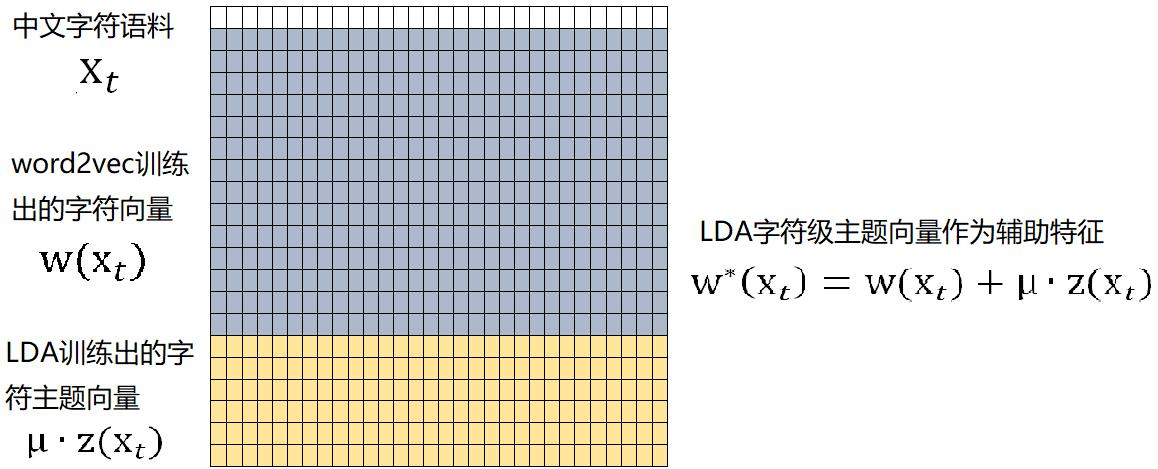
\includegraphics[width=0.95\textwidth,height=5.4cm]{./figure/主题向量拼接.jpg}
\caption{LDA主题向量作为辅助特征}
\label{lab:1}
\end{minipage}
\end{figure}

本章改进的中文字符级特征表示方法,在初始word2vec中文字符向量的基础上,为了解决一字多义,字向量空间局限的问题,采用了基于位置信息对字符向量进行优化;为了解决原模型局限于局部信息的缺点加入了全文级别的字符主题特征,结合成为一种较优的中文字符级特征表示方法,该方法及整体基于深度学习的命名实体识别模型流程图如下:

\begin{figure}[H]
\centering
\begin{minipage}[t]{\textwidth}
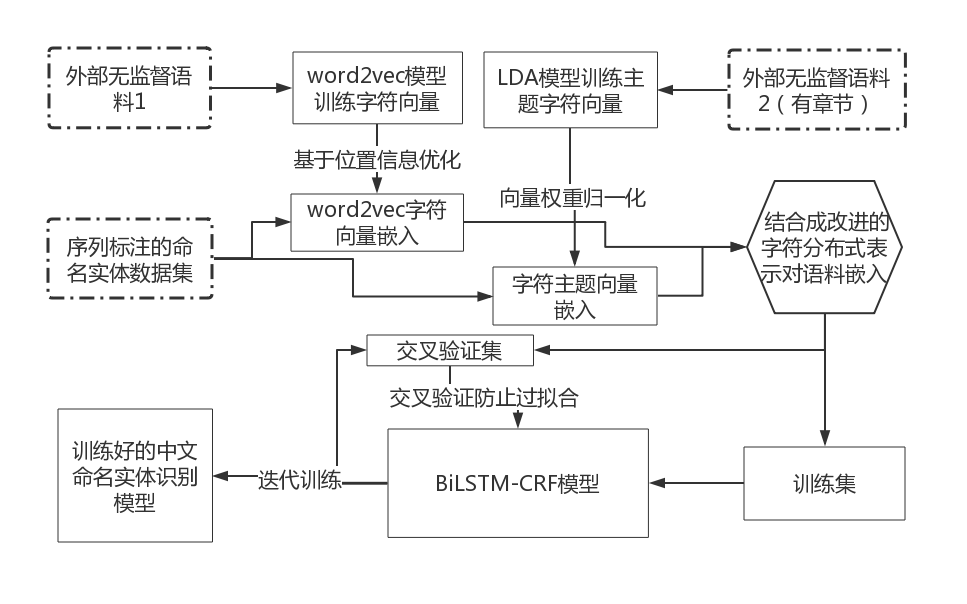
\includegraphics[width=1\textwidth,height=9.5cm]{./figure/改进的字符分布式表示.jpg}
\caption{模型流程图}
\label{lab:1}
\end{minipage}
\end{figure}

\section{实验}

\subsection{实验环境与设置}

\subsubsection{实验环境}

本文的实验主要用到实验设备主要有一台主频2.20GHz,16GB内存,处理器四核i5的个人计算机,操作系统为window,还有一台主频为2.2GHz、处理器为40核的Intel Xeon E5-2630,内存128G,操作系统为Ubun16.04的服务器。

各项实验均在Python3.6环境下编写运行,其中词向量训练、主题向量训练采用Gensim开源软件库,Gensim是一个可用于无监督主题建模和自然语言处理的开放元法库,利用现代统计机器学方法对语言建模,其对大规模语料和在线算法的支持性非常好。利用Gensim可以帮助实现Fasttext、word2vec、doc2vec、LSA、LDA、NMF、LDA、TFIDF等经典自然语言处理模型。

神经网络模型采用谷歌公司开发的开源软件库TensorFlow\cite{TensorFlow}实现.TensorFlow是一个设计用于数据流可迭代计算的开源框架,由Google Brain团队开发,支持CPU、GPU、TPU等多种设备。TensorFlow将计算表示为状态数据流图,使得深度学习的各种模型可以方便地编写运行,常见的CNN、RNN、LSTM等网络模型可以方便的开发和实现。

\subsubsection{实验数据}

(1)本文实验里中文命名实体识别数据集采用的是人民日报语料,按“BIO”标签方案标注,每个中文字符标注为{O, B-PER, I-PER, B-LOC, I-LOC, B-ORG, I-ORG}集合中的一个类别。将数据集分为训练集和测试集,训练集用来训练中文命名实体模型,测试集用来衡量模型最终的效果。训练集共有46364条语料,包括17615个人名实体,36517个地名实体,20571个组织名实体;测试集共有4365条语料,包括1973个人名实体,2877个地名实体,1331个组织名实体。

(2)本文实验中word2ve模型训练字向量的模型采用的是中文维基百科语料,共有133万余条词条,共有438530048字,涉及各类名词的定义,解释等等。

(3)本文实验中LDA模型字符主题向量训练采用的语料是腾讯新闻,共15147篇各主题的新闻,约2000万字。主题多样,包含体育、政治、娱乐、社会、财经等等话题。

\subsubsection{网络参数与训练方法}

本文实验采用的神经网络模型涉及多种参数以及各种网络训练优化方法,以下对这些内容一一介绍:

(1)网络参数

本实验BiLSTM网络模型中的参数设置如下:批处理数(batch\_size)为64;最大迭代轮次为50;隐层神经元个数为300;优化算法采用Adam\cite{Adam}(自适应时刻估计法)算法;clip梯度设置为5.0来防止训练过程中遇到梯度爆炸的情况。

(2)目标函数

目标函数设置为交叉熵函数,交叉熵函数起源于信息论中,用来衡量两种概率分布的差异,交叉熵的定义为:概率分布p和概率分布q的交叉熵为:

\begin{equation}
H(p, q)=E_{p}[-\log q]=H(p)+D_{K L}(p \| q)
\end{equation}

其中$H(p)$是p的熵,$D_{K L}(p \| q)$是从p到q的KL散度。对于本文的离散情况,四散分布p和q的交叉熵为:

\begin{equation}
H(p, q)=-\sum_{x} p(x) \log q(x)
\end{equation}

在训练的过程中,用该次迭代的批处理数据通过网络计算出预测结果,计算预测结果与真实结果间的交叉熵,做为本轮迭代的损失,根据反向传播算法对神经网络中的参数进行调整。

(3)Xavier初始化

在深度学习过程中,各层神经元不能初始化为0,不然将会遭遇梯度为0的情况。因而要对神经元初始化,Xavier初始化由\cite{Glorot}提出,思路是将初始化应该使得各层的激活值和状态梯度的方差在传播过程中的方差保持一致,这样的初始化方式可以使得神经网络在向前传播时神经元输出值的方差不会不断增大,有较强的稳定性。

(4)随机失活(Dropout)

随机失活这种网络训练方法,借鉴正则化的思想,对随机失活作用下的一层节点,对每个节点设置一个节点保留概率,取值在0到1之间,在训练时按概率超过设置阈值时失活。这样的方法使得神经网络不会过于偏向某一个节点,从而是的单个节点的权重不会过大。本实验中对所有神经网络层都采取这一优化训练的方法。

(5)shuffle

shuffle方法是在每轮迭代前将训练集重新排序,使得这些例子能够被随机分配到不同的batches中。这样的方法可以使数据更加混乱,防止网络的过拟合,让模型训练的效果更好。本实验在每轮迭代前通过shuffle方法随机打乱训练集。

(6)早停(Earlystop)

模型迭代的次数太长的话会造成网络对于训练集过拟合,即在训练集上表现越来越好,但是在其他数据集上表现越来越差。训练模型时往往没有到达最大迭代次数时就可以提前结束训练数据,保存模型往往能达到在总体数据上较好的表现,这样的方法就叫做早停策略。利用这样的方法,每隔一段训练次数用交叉验证集测试当年模型的效果,当模型在交叉验证集上长时间效果不再提升甚至有下降的趋势时提前停止训练,保存模型。

\subsection{实验结果与分析}

(1)基准模型效果

利用训练语料训练出100维中文字符向量,嵌入后通过双向长短时记忆网络和条件随机场进行训练,得到CharEmbedding-BiLSTM-CRF模型。

\begin{table}[H]
\centering
\begin{tabular}{|l|l|l|l|}
\hline
    & 准确率     & 召回率     & F值    \\ \hline
LOC & 92.60\% & 88.67\% & 90.59 \\ \hline
ORG & 83.78\% & 84.22\% & 84.00 \\ \hline
PER & 86.29\% & 82.46\% & 84.33 \\ \hline
整体  & 88.63\% & 85.72\% & 87.15 \\ \hline
\end{tabular}
\caption{CharEmbedding-BiLSTM-CRF模型实验结果}
\end{table}

表3-4是CharEmbedding-BiLSTM-CRF模型的实验结果,该模型对于中文命名识别有较优的效果。同时观察不同类别实体的识别准确度召回度,也能看出模型对于地名的识别较为准确,对于人名、组织名的识别较差。因为地名重复性强,而人名组织名重组复杂性高很多,这两类实体也是模型待提高的要点。

(2)基于位置信息优化方法实验与分析

根据3.4节内容,基于位置信息优化中文字符向量的方法涉及到偏移参数的寻找,我们采用网格搜索的方法找出较优的参数。当只考虑$x_{t}$前后k个字符的信息时,取不同的$\lambda$值时,效果如下:




(3)基于主题信息的构造方法实验与分析




(4)整体改进中文字符特征方法的实验与分析




\section{本章小结}

\chapter{面向复杂命名实体识别的层次深度神经网络模型}

\section{引言}

\section{复杂命名实体概述与相关工作}

英文:

中文:
中文嵌套命名实体关系抽取研究 许浩亮



\section{层次标签与层次深度神经网络模型构建}

\section{实验及结果分析}

\section{本章小结}

\chapter{中文复杂命名实体识别在企业风险识别中的应用}

\section{引言}

\section{应用背景}

\section{数据爬虫}

\section{文本分类模块}

\section{命名实体识别模块}

\section{企业风险识别}

\chapter{总结与展望}

\section{工作总结}

\section{不足与展望}

基于位置信息不足,因字符调整比如tf-idf从词频角度出发,非对称模型




%%%%%%%%%%%%%%%%%%%%%%%%%%%%%%%%%%%%%%%%%%%%%%%%%%%%%%%%%%%%%%%%%%%%%%%%%%%%%%%
% 致谢,应放在《结论》之后
\begin{acknowledgement}
%thanks
时光荏苒,在南京大学的本科的学习生活即将结束,四年的时间转瞬即逝,这几年的经历必将成为我人生宝贵的财富。在此论文完成之际,谨向这几年来帮助我的老师和同学表达最衷心的感

\end{acknowledgement}

%%%%%%%%%%%%%%%%%%%%%%%%%%%%%%%%%%%%%%%%%%%%%%%%%%%%%%%%%%%%%%%%%%%%%%%%%%%%%%%




% 参考文献。应放在\backmatter之前。
% 推荐使用BibTeX,若不使用BibTeX时注释掉下面一句。
%\nocite{*}
\bibliography{sample}


% 附录,必须放在参考文献后,backmatter前
\appendix
\chapter{MPTCP内核源代码修改}\label{app:1}
\section{函数mptcp\_v4\_subflows()}
\begin{lstlisting}[language=C]
static void mptcp_v4_subflows(struct sock *meta_sk, const struct mptcp_loc4 *loc, struct mptcp_rem4 *rem)
{
   int i;
   int num;
   printk(KERN_INFO "******** Entering mptcp_v4_subflows ********\n");

   initial_my_global_var();
   switch(my_counter)
   {
		case 1 : num = Fir; break;
		case 2 : num = Sec; break;
		case 3 : num = Thi; break;
		default : num = Fir;
	}

	for (i = 1; i < num; i++)
	{
		printk(KERN_INFO "******** in mptcp_v4_subflows i = %d num = %d********\n",i,num);
		mptcp_init4_subsockets(meta_sk, loc, rem);
	}
	printk(KERN_INFO "******** Leaving mptcp_v4_subflows ********\n");
}
\end{lstlisting}

%%%%%%%%%%%%%%%%%%%%%%%%%%%%%%%%%%%%%%%%%%%%%%%%%%%%%%%%%%%%%%%%%%%%%%%%%%%%%%%
% 书籍附件
\backmatter
%%%%%%%%%%%%%%%%%%%%%%%%%%%%%%%%%%%%%%%%%%%%%%%%%%%%%%%%%%%%%%%%%%%%%%%%%%%%%%%
% 作者简历与科研成果页,应放在backmatter之后
\begin{resume}
% 论文作者身份简介,一句话即可。
\begin{authorinfo}
\noindent 韦小宝,男,汉族,1985年11月出生,江苏省扬州人。
\end{authorinfo}
% 论文作者教育经历列表,按日期从近到远排列,不包括将要申请的学位。
\begin{education}
\item[2007年9月 --- 2010年6月] 南京大学计算机科学与技术系 \hfill 硕士
\item[2003年9月 --- 2007年6月] 南京大学计算机科学与技术系 \hfill 本科
\end{education}
% 论文作者在攻读学位期间所发表的文章的列表,按发表日期从近到远排列。
\begin{publications}
\item Xiaobao Wei, Jinnan Chen, ``Voting-on-Grid Clustering for Secure
  Localization in Wireless Sensor Networks,'' in \textsl{Proc. IEEE International
    Conference on Communications (ICC) 2010}, May. 2010.
\item Xiaobao Wei, Shiba Mao, Jinnan Chen, ``Protecting Source Location Privacy
  in Wireless Sensor Networks with Data Aggregation,'' in \textsl{Proc. 6th
    International Conference on Ubiquitous Intelligence and Computing (UIC)
    2009}, Oct. 2009.
\end{publications}
% 论文作者在攻读学位期间参与的科研课题的列表,按照日期从近到远排列。
\begin{projects}
\item 国家自然科学基金面上项目``无线传感器网络在知识获取过程中的若干安全问题研究''
(课题年限~2010年1月 --- 2012年12月),负责位置相关安全问题的研究。
\item 江苏省知识创新工程重要方向项目下属课题``下一代移动通信安全机制研究''
(课题年限~2010年1月 --- 2010年12月),负责LTE/SAE认证相关的安全问题研究。
\end{projects}
\end{resume}

%%%%%%%%%%%%%%%%%%%%%%%%%%%%%%%%%%%%%%%%%%%%%%%%%%%%%%%%%%%%%%%%%%%%%%%%%%%%%%%
% 生成《学位论文出版授权书》页面,应放在最后一页
%\makelicense

%%%%%%%%%%%%%%%%%%%%%%%%%%%%%%%%%%%%%%%%%%%%%%%%%%%%%%%%%%%%%%%%%%%%%%%%%%%%%%%
\end{document}
